\documentclass{beamer}

\usepackage{color}
\usepackage{multirow} %used for crazy tables
\usepackage{stmaryrd} %used for /shortrightarrow
\usepackage{array} %used for \setlength\extrarowheight
%usepackage{psfig}

\usepackage{graphicx}
\usepackage{verbatim}
\usepackage{amsmath}
\usepackage{amssymb}
\usepackage{xy}
\usepackage{color}

\usepackage{epsfig}

\usepackage{etex}

\usepackage{geometry}
\usepackage{hyperref}
\usepackage{media9}
%\usepackage{movie15} 

\usepackage{beamerprosper}
\usepackage{ifthen}
\newboolean{fullDocument}
\setboolean{fullDocument}{true}
%\setboolean{fullDocument}{false}

\xyoption{all}
\xyoption{graph}
\xyoption{poly}

\usepackage{textcomp}
\usepackage{graphics}
\usepackage{wasysym}


\newcommand{\rbs}{*+[F=:<10pt>]{~~~~~}}
\newcommand{\pr}{\Rsh}
\newcommand{\bbid}[1]{\rotatebox{90}{#1}}
\newcommand{\gene}[1]{*+[F*]{\txt{#1}}}
\newcommand{\trm}{\octagon}
\newcommand{\twotrm}{\octagon \octagon}
\newcommand{\ckt}{\save}
\newcommand{\eckt}{\POS *++[F--:<5pt>]\frm{} \restore}

%\newcommand{\red}[1]{\textcolor{red}{#1}}

\definecolor{myRed}{rgb}{0.85,0,0.13}

\mode<presentation>
{
  %\usetheme{AnnArbor}
  %\usetheme{Annecy}
  %\usetheme{boxes}
  %\usetheme{Frankfurt} %- 
  \usetheme{Madridsrl} %- 
  %\usetheme{Rochester}
  %\usetheme{Antibes}
  %\usetheme{CambridgeUS}
  %\usetheme{Goettingen}
  %\usetheme{Malmoe}
  %\usetheme{Singapore}
  %\usetheme{Bergen}
  %\usetheme{Copenhagen}
  %\usetheme{Hannover}
  %\usetheme{Marburg}
  %\usetheme{Szeged}
  %\usetheme{Berkeley}
  %\usetheme{Darmstadt}
  %\usetheme{Ilmenau}
  %\usetheme{Montpellier}
  %\usetheme{Warsaw}
  %\usetheme{Berlin}
  %\usetheme{default}
  %\usetheme{JuanLesPins}
  %\usetheme{PaloAlto}
  %\usetheme{Boadilla}
  %\usetheme{Dresden}
  %\usetheme{Luebeck}
  %\usetheme{Pittsburgh}

  %\usecolortheme{seahorse}
  %\usecolortheme{rose}

%setup the color scheme
%\setbeamercolor*{structure}{fg=blue!25!white}
\setbeamercolor*{structure}{fg=myRed}
%whale
\setbeamercolor*{palette primary}{use=structure,fg=white,bg=structure.fg}
\setbeamercolor*{palette secondary}{use=structure,fg=white,bg=structure.fg!75!black}
\setbeamercolor*{palette tertiary}{use=structure,fg=white,bg=structure.fg!50!black}
\setbeamercolor*{palette quaternary}{fg=white,bg=black}

\setbeamercolor*{sidebar}{use=structure,bg=structure.fg}
  
\setbeamercolor*{palette sidebar primary}{use=structure,fg=structure.fg!10}
\setbeamercolor*{palette sidebar secondary}{fg=white}
\setbeamercolor*{palette sidebar tertiary}{use=structure,fg=structure.fg!50}
\setbeamercolor*{palette sidebar quaternary}{fg=white}

\setbeamercolor*{titlelike}{parent=palette primary}

\setbeamercolor*{separation line}{}
\setbeamercolor*{fine separation line}{}

%orchid
\setbeamercolor{block title}{use=structure,fg=white,bg=structure.fg!75!black}
\setbeamercolor{block title alerted}{use=alerted text,fg=white,bg=alerted text.fg!75!black}
\setbeamercolor{block title example}{use=example text,fg=white,bg=example text.fg!75!black}

\setbeamercolor{block body}{parent=normal text,use=block title,bg=block title.bg!10!bg}
\setbeamercolor{block body alerted}{parent=normal text,use=block title alerted,bg=block title alerted.bg!10!bg}
\setbeamercolor{block body example}{parent=normal text,use=block title example,bg=block title example.bg!10!bg}

  % or ...

  %\setbeamercovered{transparent}
  % or whatever (possibly just delete it)
  \setbeamertemplate{navigation symbols}{}

%change the logo placement
%\setbeamertemplate{sidebar right} {
%  %\vfill%
%  \llap{\insertlogo\hskip0.1cm}%
%  \vskip2pt%
%  \llap{\usebeamertemplate***{navigation symbols}\hskip0.1cm}%
%  \vskip2pt%
%
%}

\setbeamertemplate{frametitle}[default][center]{}
}

\usepackage{pslatex}
\usepackage{ulem} %for strike through \soutw
\normalem %to 'undo' the underlining of \emph in ulem
\usepackage[english]{babel}
% or whatever

\usepackage[latin1]{inputenc}
% or whatever

\usepackage{times}
\usepackage[T1]{fontenc}
\usepackage{multirow}
% Or whatever. Note that the encoding and the font should match. If T1
% does not look nice, try deleting the line with the fontenc.
\usepackage{tabularx}
\newcolumntype{C}{>{\centering\arraybackslash}p{0.45\textwidth}}

\def\algorithm{\bgroup\obeylines\obeyspaces\def\ {\quad}
\footnotesize\tt\leftskip=2pc\vskip4pt\relax}
\def\endalgorithm{\vskip4pt\egroup}

\def\myspecies{S}
\def\experiments{E}
\def\experiment{\delta}
\def\weights{W}
\def\datapoint{\alpha}
\def\time{\tau}
\def\vector{\nu}
\def\edges{C}
\def\info{I}
\def\thresholds{T}
\def\suchthat{\ni}
\def\mutated{M}
\def\levels{L}

\newcommand{\wh}[1]{\textcolor{white}{#1}}
\newcommand{\red}[1]{\textcolor{red}{#1}}
\newcommand{\blue}[1]{\textcolor{blue}{#1}}
\newcommand{\green}[1]{\textcolor{green}{#1}}

\title[A Brief History of COMBINE]{A Brief History of COMBINE}

\author[Chris J. Myers et al.]{Chris J. Myers, Gary Bader, Padraig Gleeson, Martin Golebiewski, \\ 
Michael Hucka, Nicolas Le Nov\`{e}re, David P. Nickerson, Falk Schreiber, \\
and Dagmar Waltemath}

\institute[COMBINE]{\textcolor{red}{\normalsize COMBINE}}

\date[WSC 2017 / December 5, 2017]{\textcolor{blue}{Winter Simulation 2017}\\December 5, 2017}

\begin{document}

\begin{frame}
  \titlepage
\end{frame}

\begin{frame}\frametitle{Reproducibility Crisis}
\begin{center}
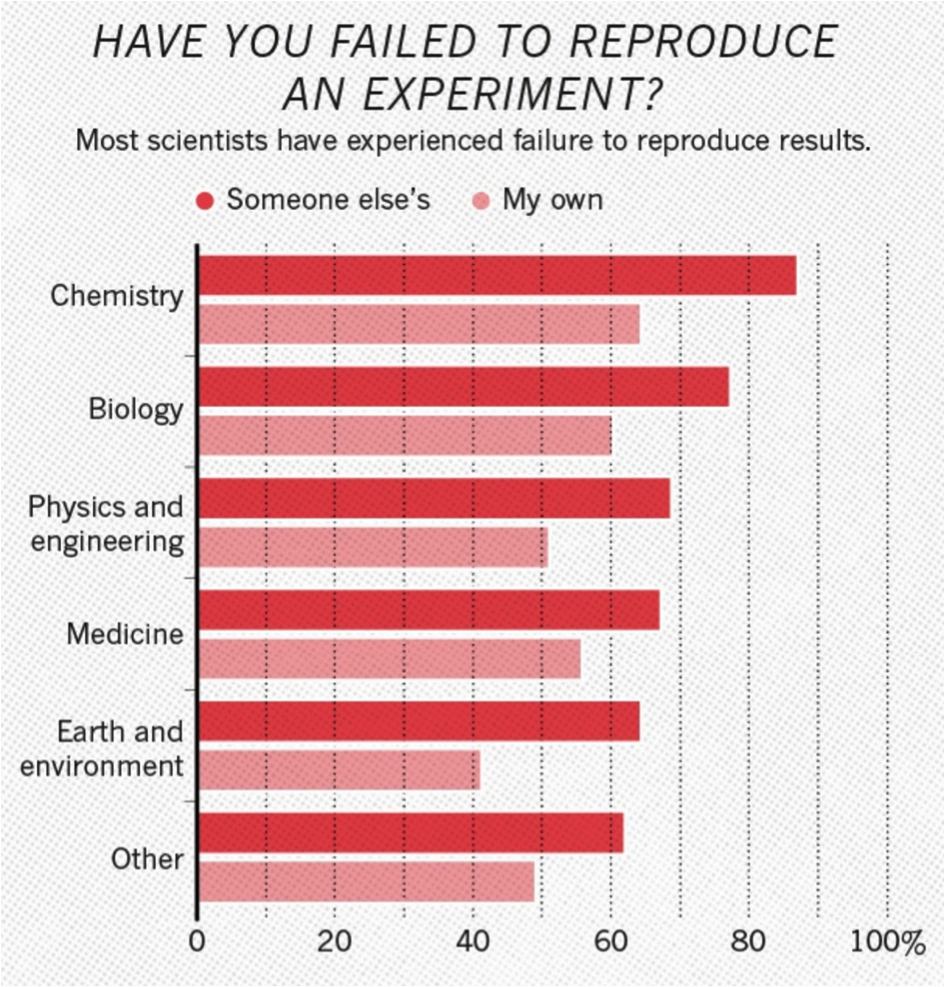
\includegraphics[width=0.575\textwidth]{figs/FailureToReproduce}\\
{\footnotesize (V. Simonyan, Center for Biologics Evaluation and Research FDA, USA)}
\end{center}
\end{frame}

\begin{frame}\frametitle{Reproducibility Crisis}
\begin{center}
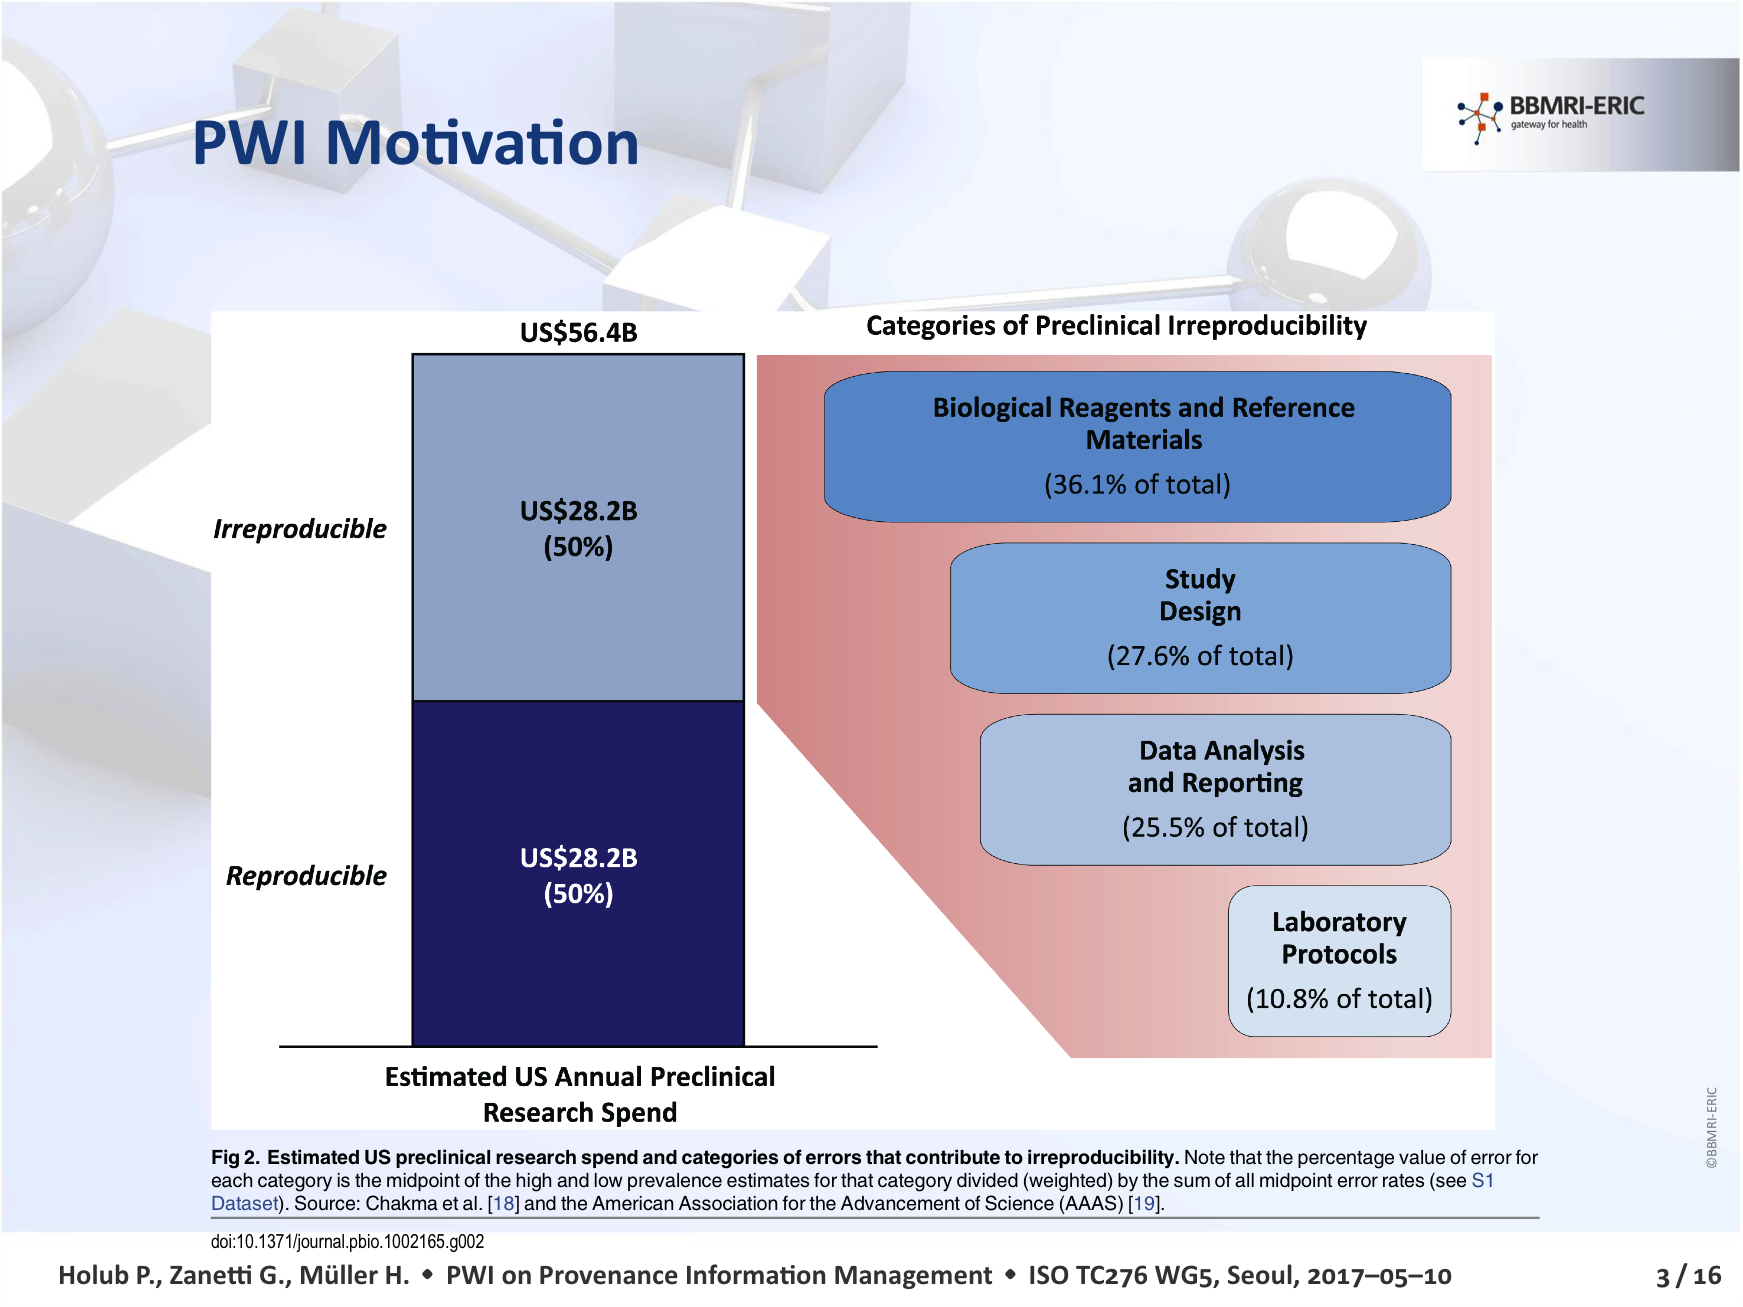
\includegraphics[width=0.85\textwidth]{figs/FailureToReproduce2}
\end{center}
\end{frame}

\begin{frame}\frametitle{Reproducibility Crisis}
\begin{center}
\only<1>{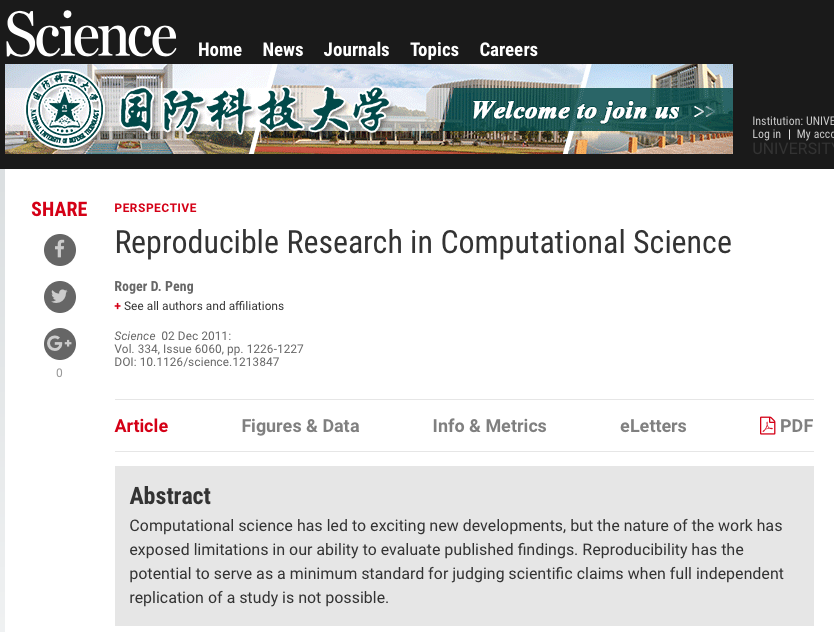
\includegraphics[width=0.8\textwidth]{figs/compReproduce2}}
\only<2>{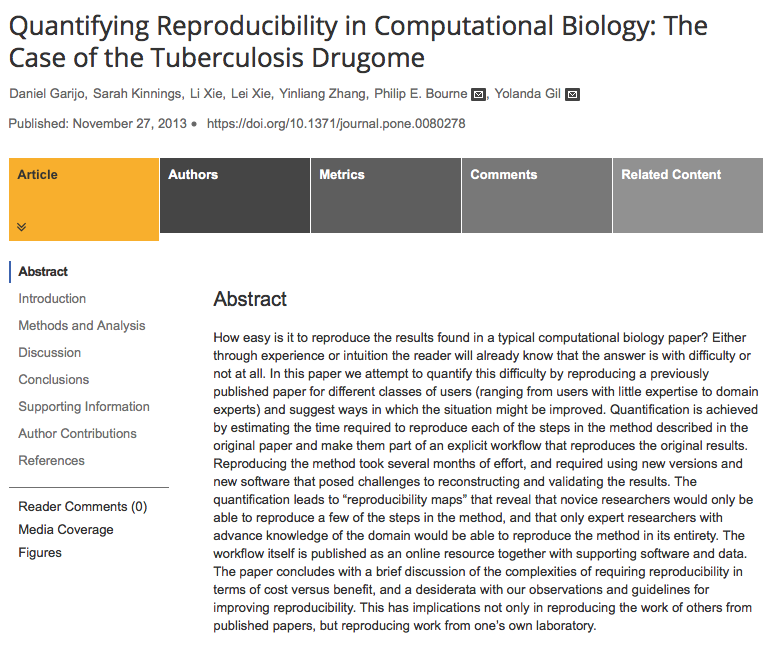
\includegraphics[width=0.8\textwidth]{figs/compReproduce}}
\only<3>{
\begin{quotation}
An article about computational science in a scientific publication is not the scholarship itself, it is merely advertising of the scholarship. The actual scholarship is the complete ... set of instructions [and data] which generated the figures.\\
-- David Donoho, 1998
\end{quotation}
}
\end{center}
\end{frame}

\begin{frame}\frametitle{Standards to the Rescue}
\begin{center}
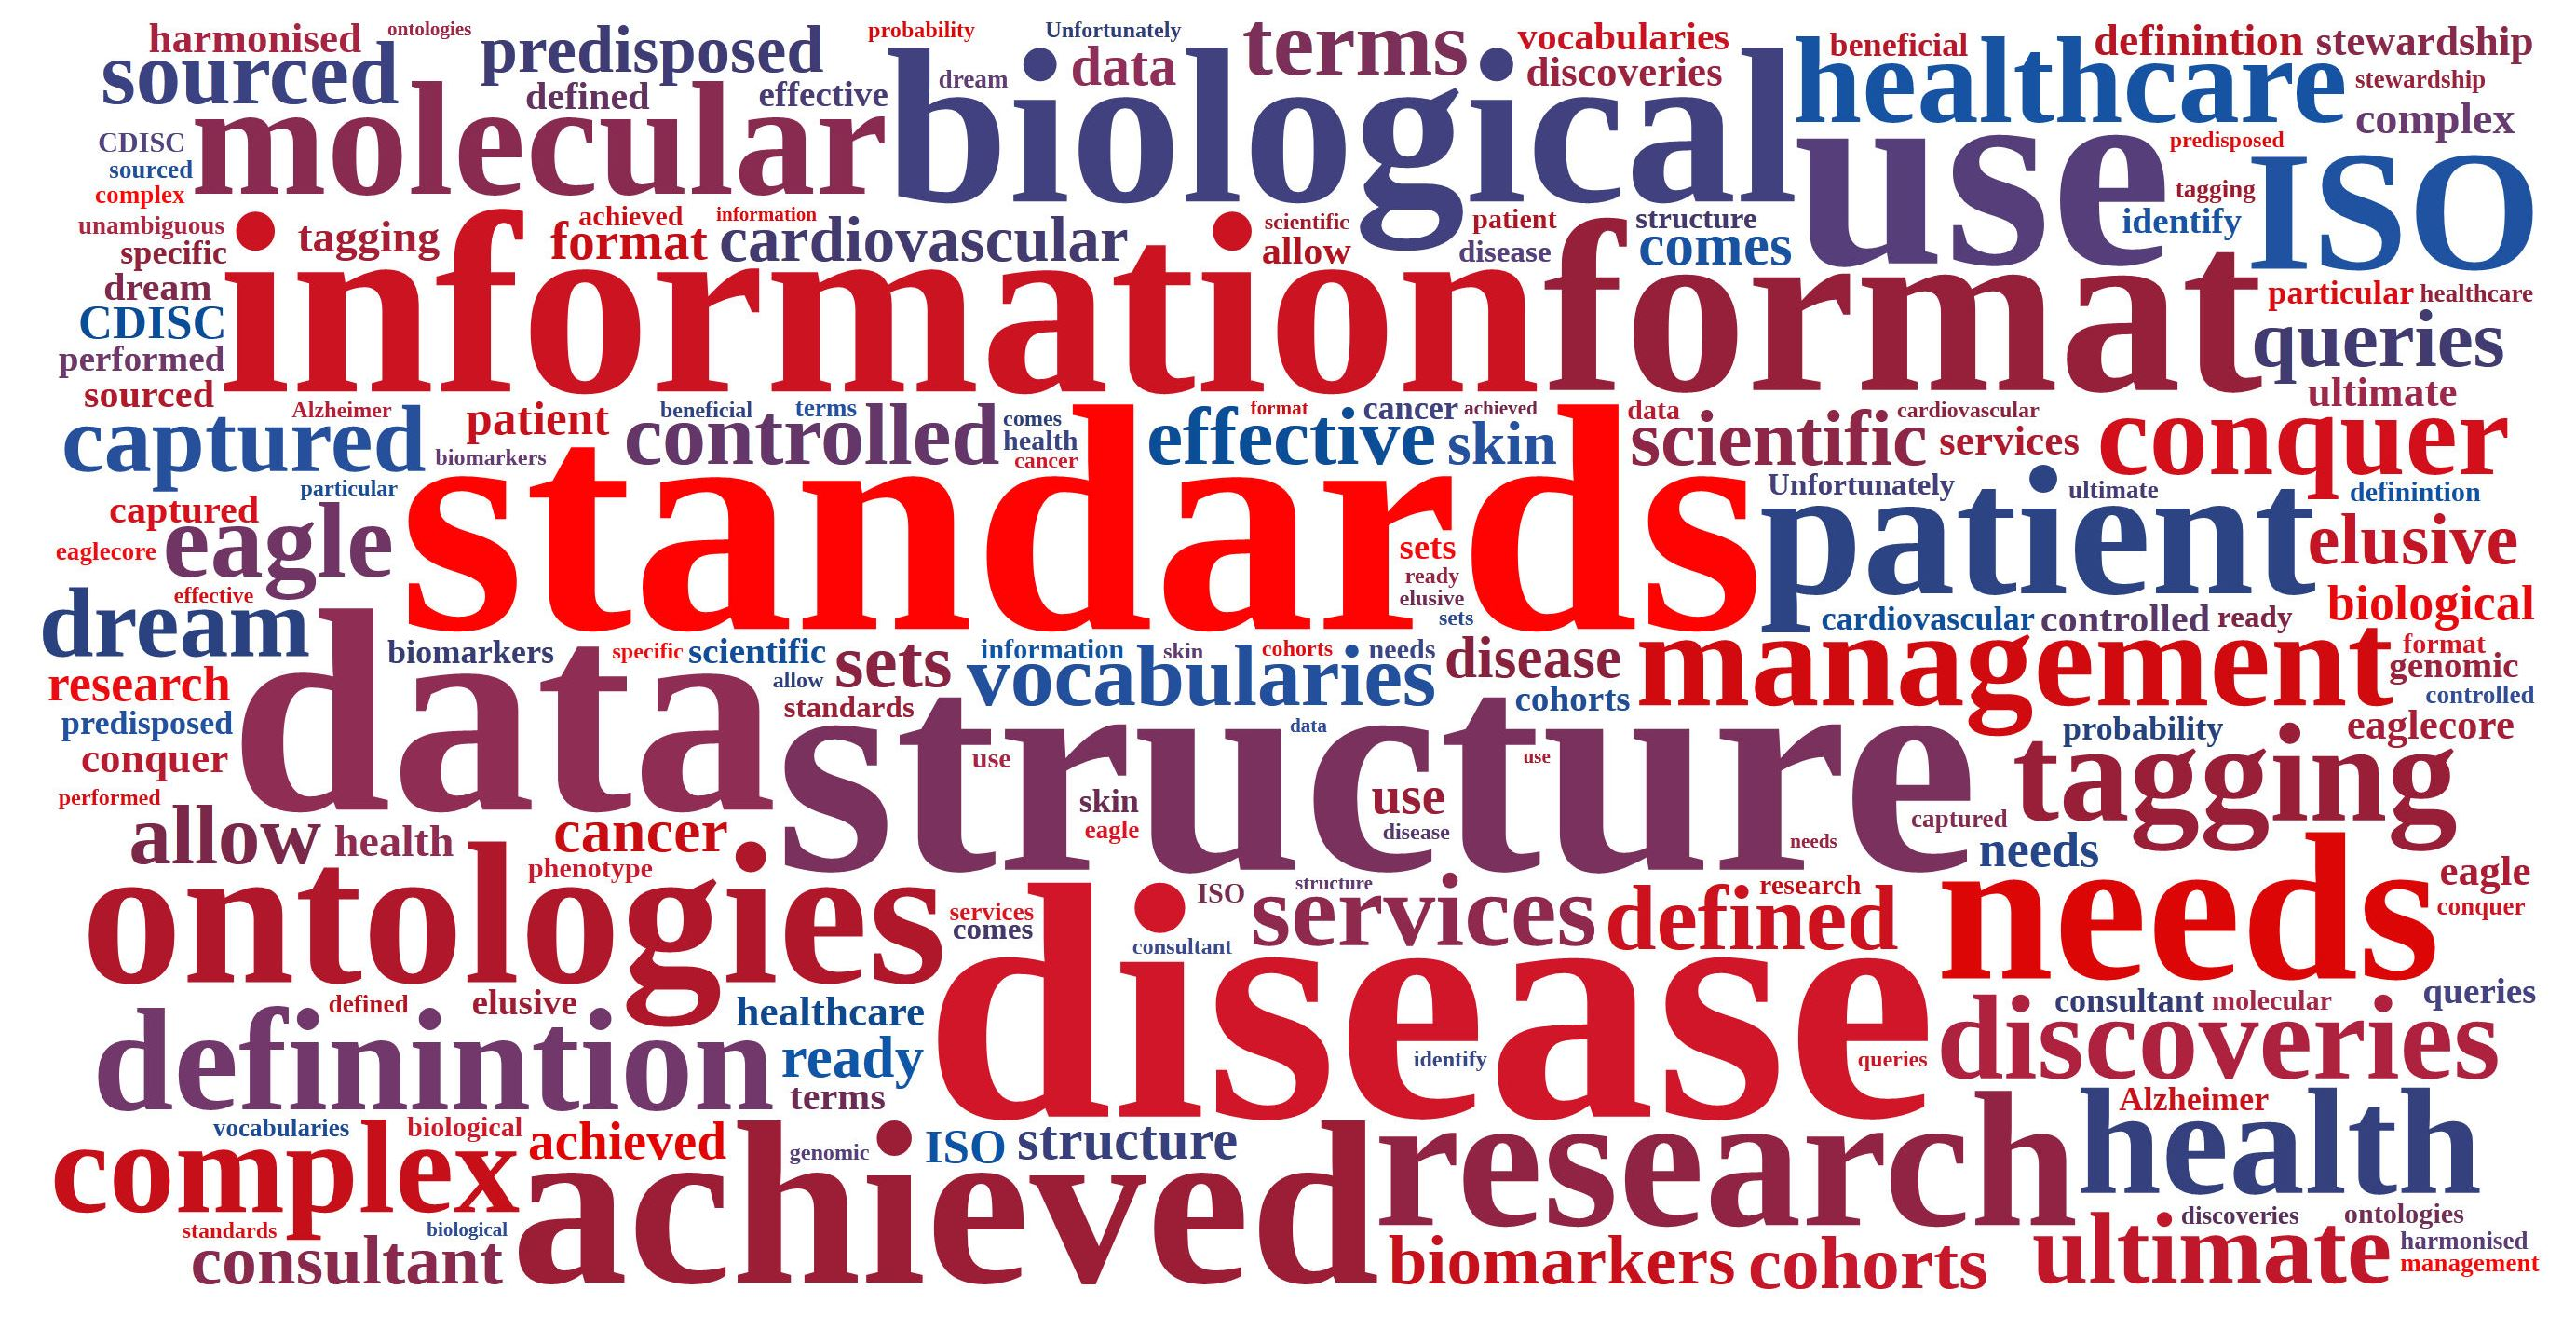
\includegraphics[width=\textwidth]{figs/standards-cloud}\\
{\footnotesize (source \url{https://www.eaglegenomics.com/do-data-standards-really-matter/})}
\end{center}
\end{frame}

\begin{frame}\frametitle{Word of Warning}
\begin{center}

\includegraphics[width=\textwidth]{figs/XKCD}\\
(source \url{xkcd.com})
\end{center}
\end{frame}

\begin{frame}\frametitle{Coordination of Standard Development\\ in Systems/Synthetic Biology}
\begin{center}

\includegraphics[width=\textwidth]{figs/COMBINE}\\
{\LARGE \url{http://co.mbine.org}}
\end{center}
\begin{itemize}
\item Tasks and Actions:
\begin{itemize}
\item Computational Modeling in Biology Network
\item Concerted meetings of standards: HARMONY \& the COMBINE Forum
\item Training in application of standards (COMBINE tutorials)
\item Coordinate standards development
\item Develop common procedures \& tools
\item Provide a recognized voice
\end{itemize}
\end{itemize}
\end{frame}

%% \begin{frame}\frametitle{COMBINE Community}
%% \begin{center}
%% %
\includegraphics[width=\textwidth]{figs/XKCD}\\
%% %(source \url{xkcd.com})
%% \end{center}
%% \end{frame}

\begin{frame}\frametitle{COMBINE History}
\begin{center}
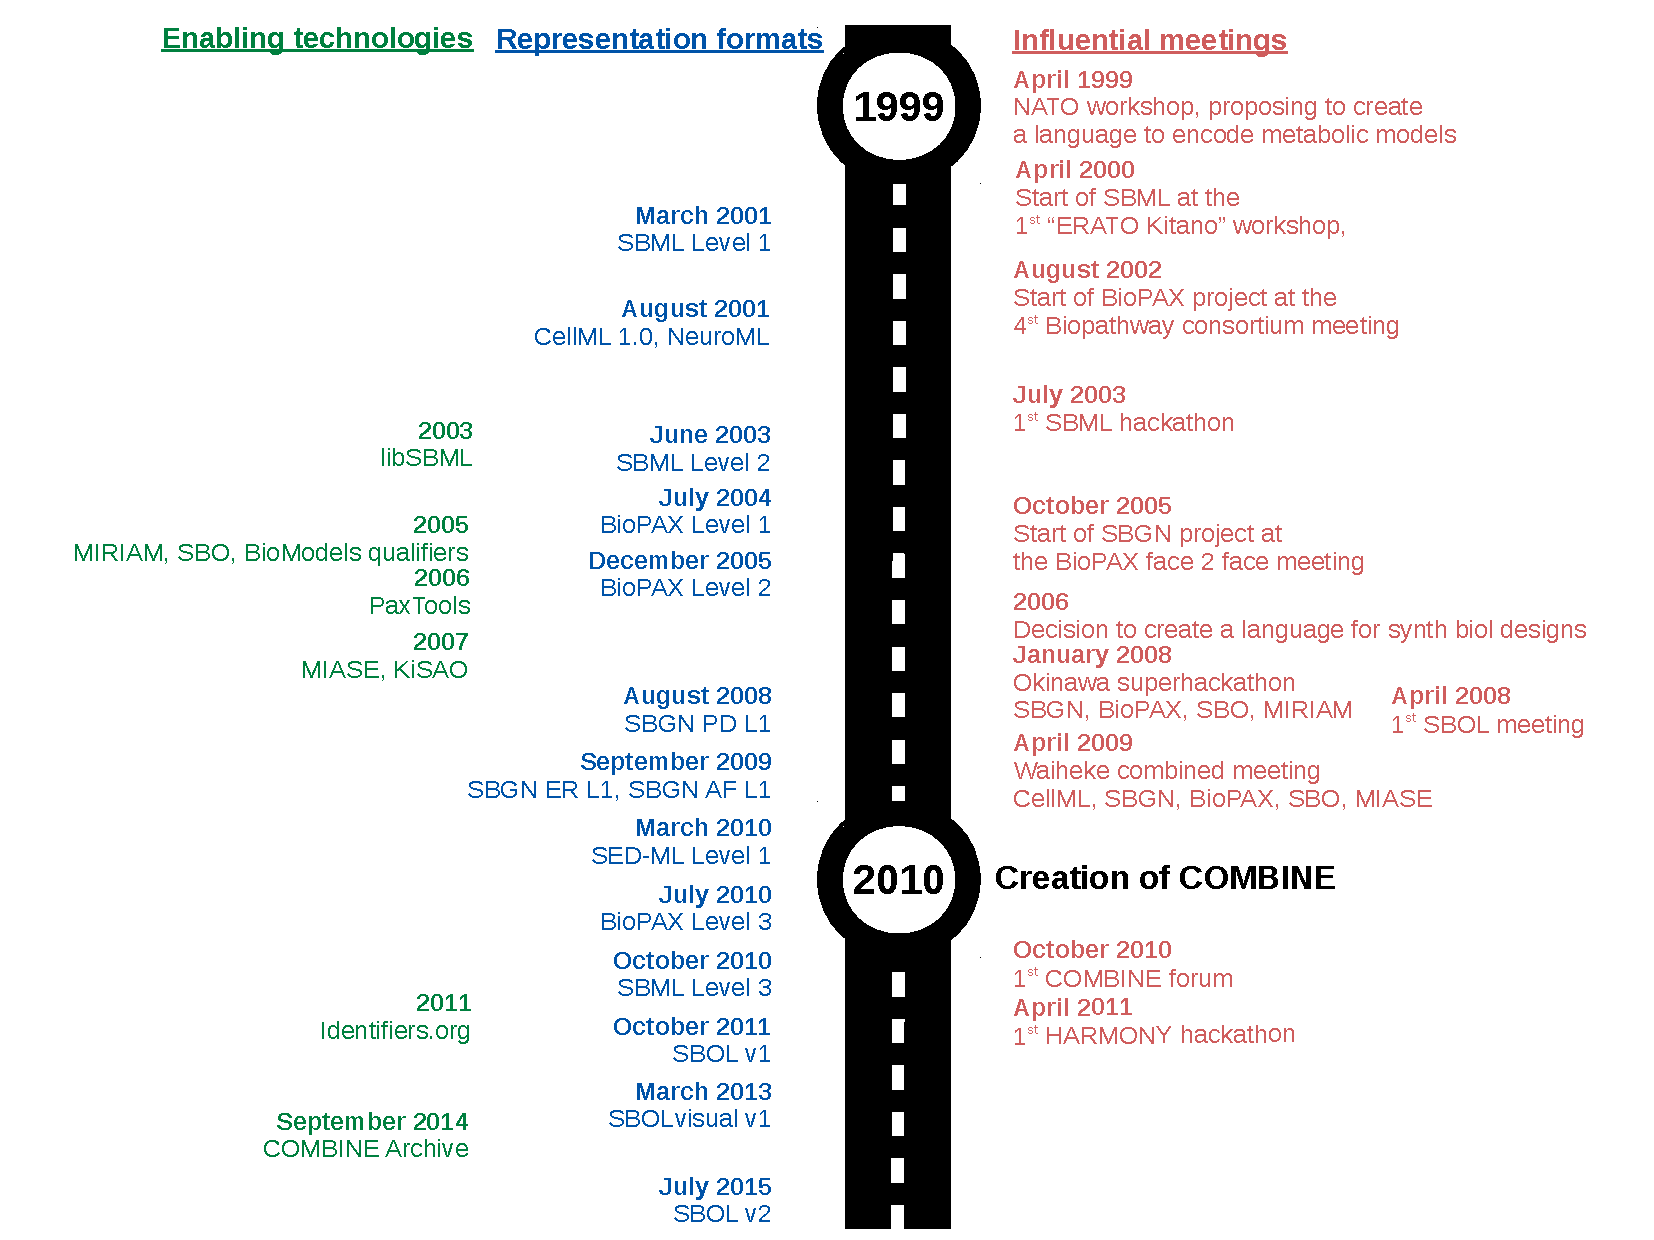
\includegraphics[width=0.85\textwidth]{figs/COMBINE-history}
\end{center}
\end{frame}

\begin{frame}\frametitle{COMBINE Overview}
\begin{center}
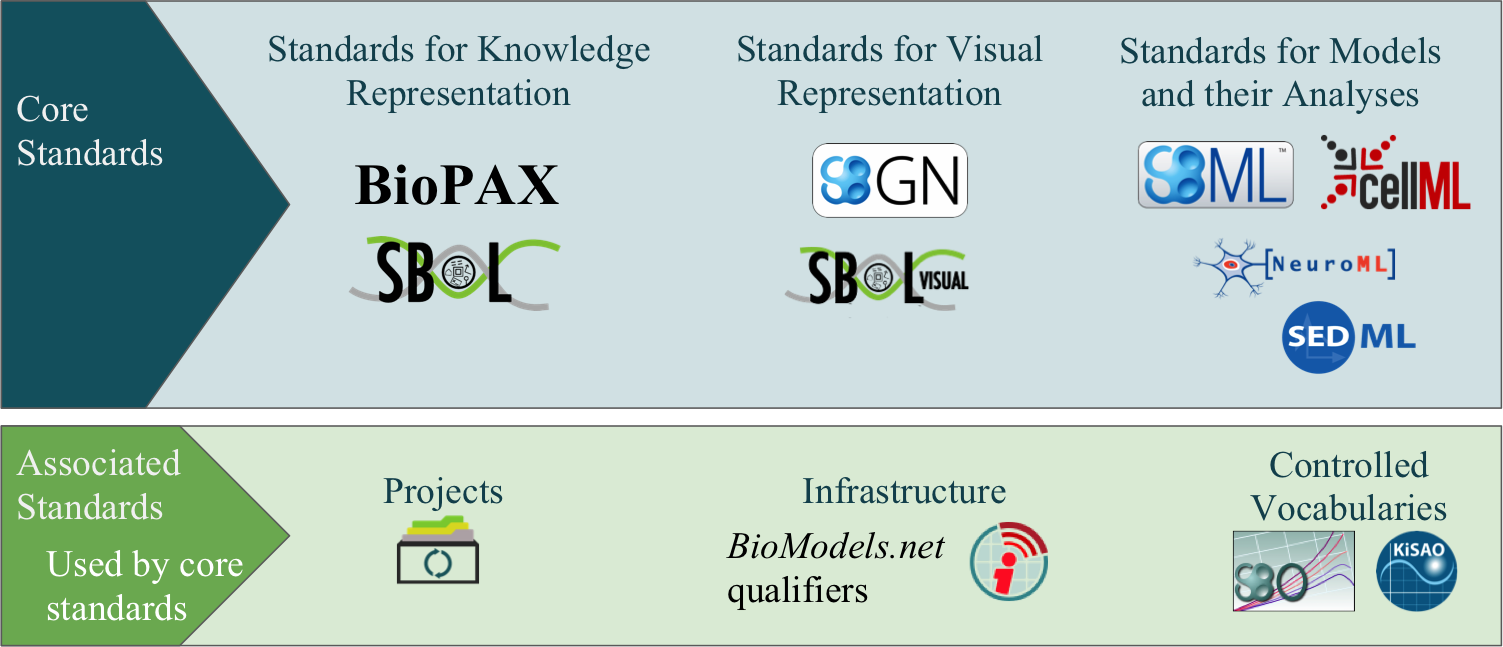
\includegraphics[width=\textwidth]{figs/COMBINE_Overview3}
\end{center}
\end{frame}

\begin{frame}\frametitle{BioPax: Biological Pathways}
\begin{center}
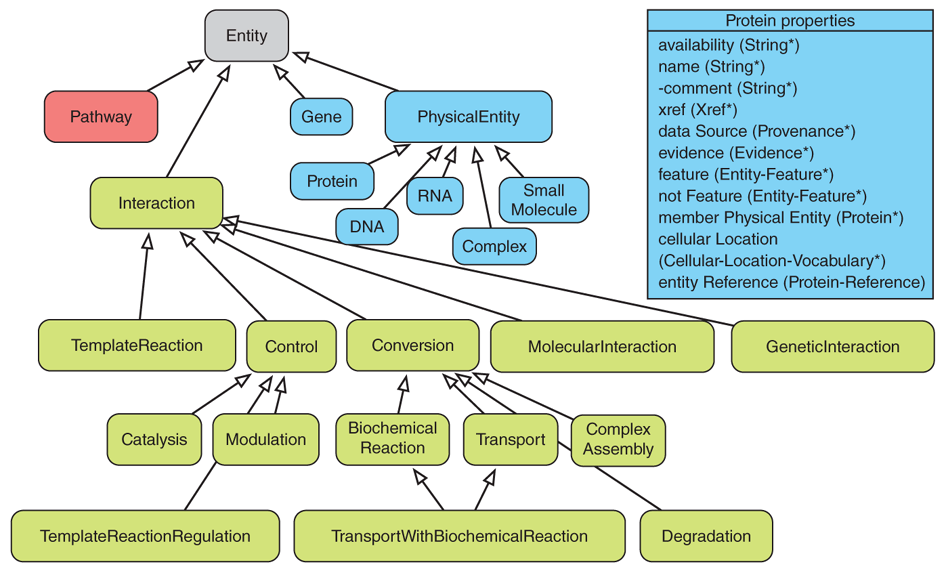
\includegraphics[width=\textwidth]{figs/BioPax}\\
Demir et al., Nature Biotechnlogy (2010)
\end{center}
\end{frame}

\begin{frame}\frametitle{Synthetic Biology Open Language (SBOL)}
\begin{center}
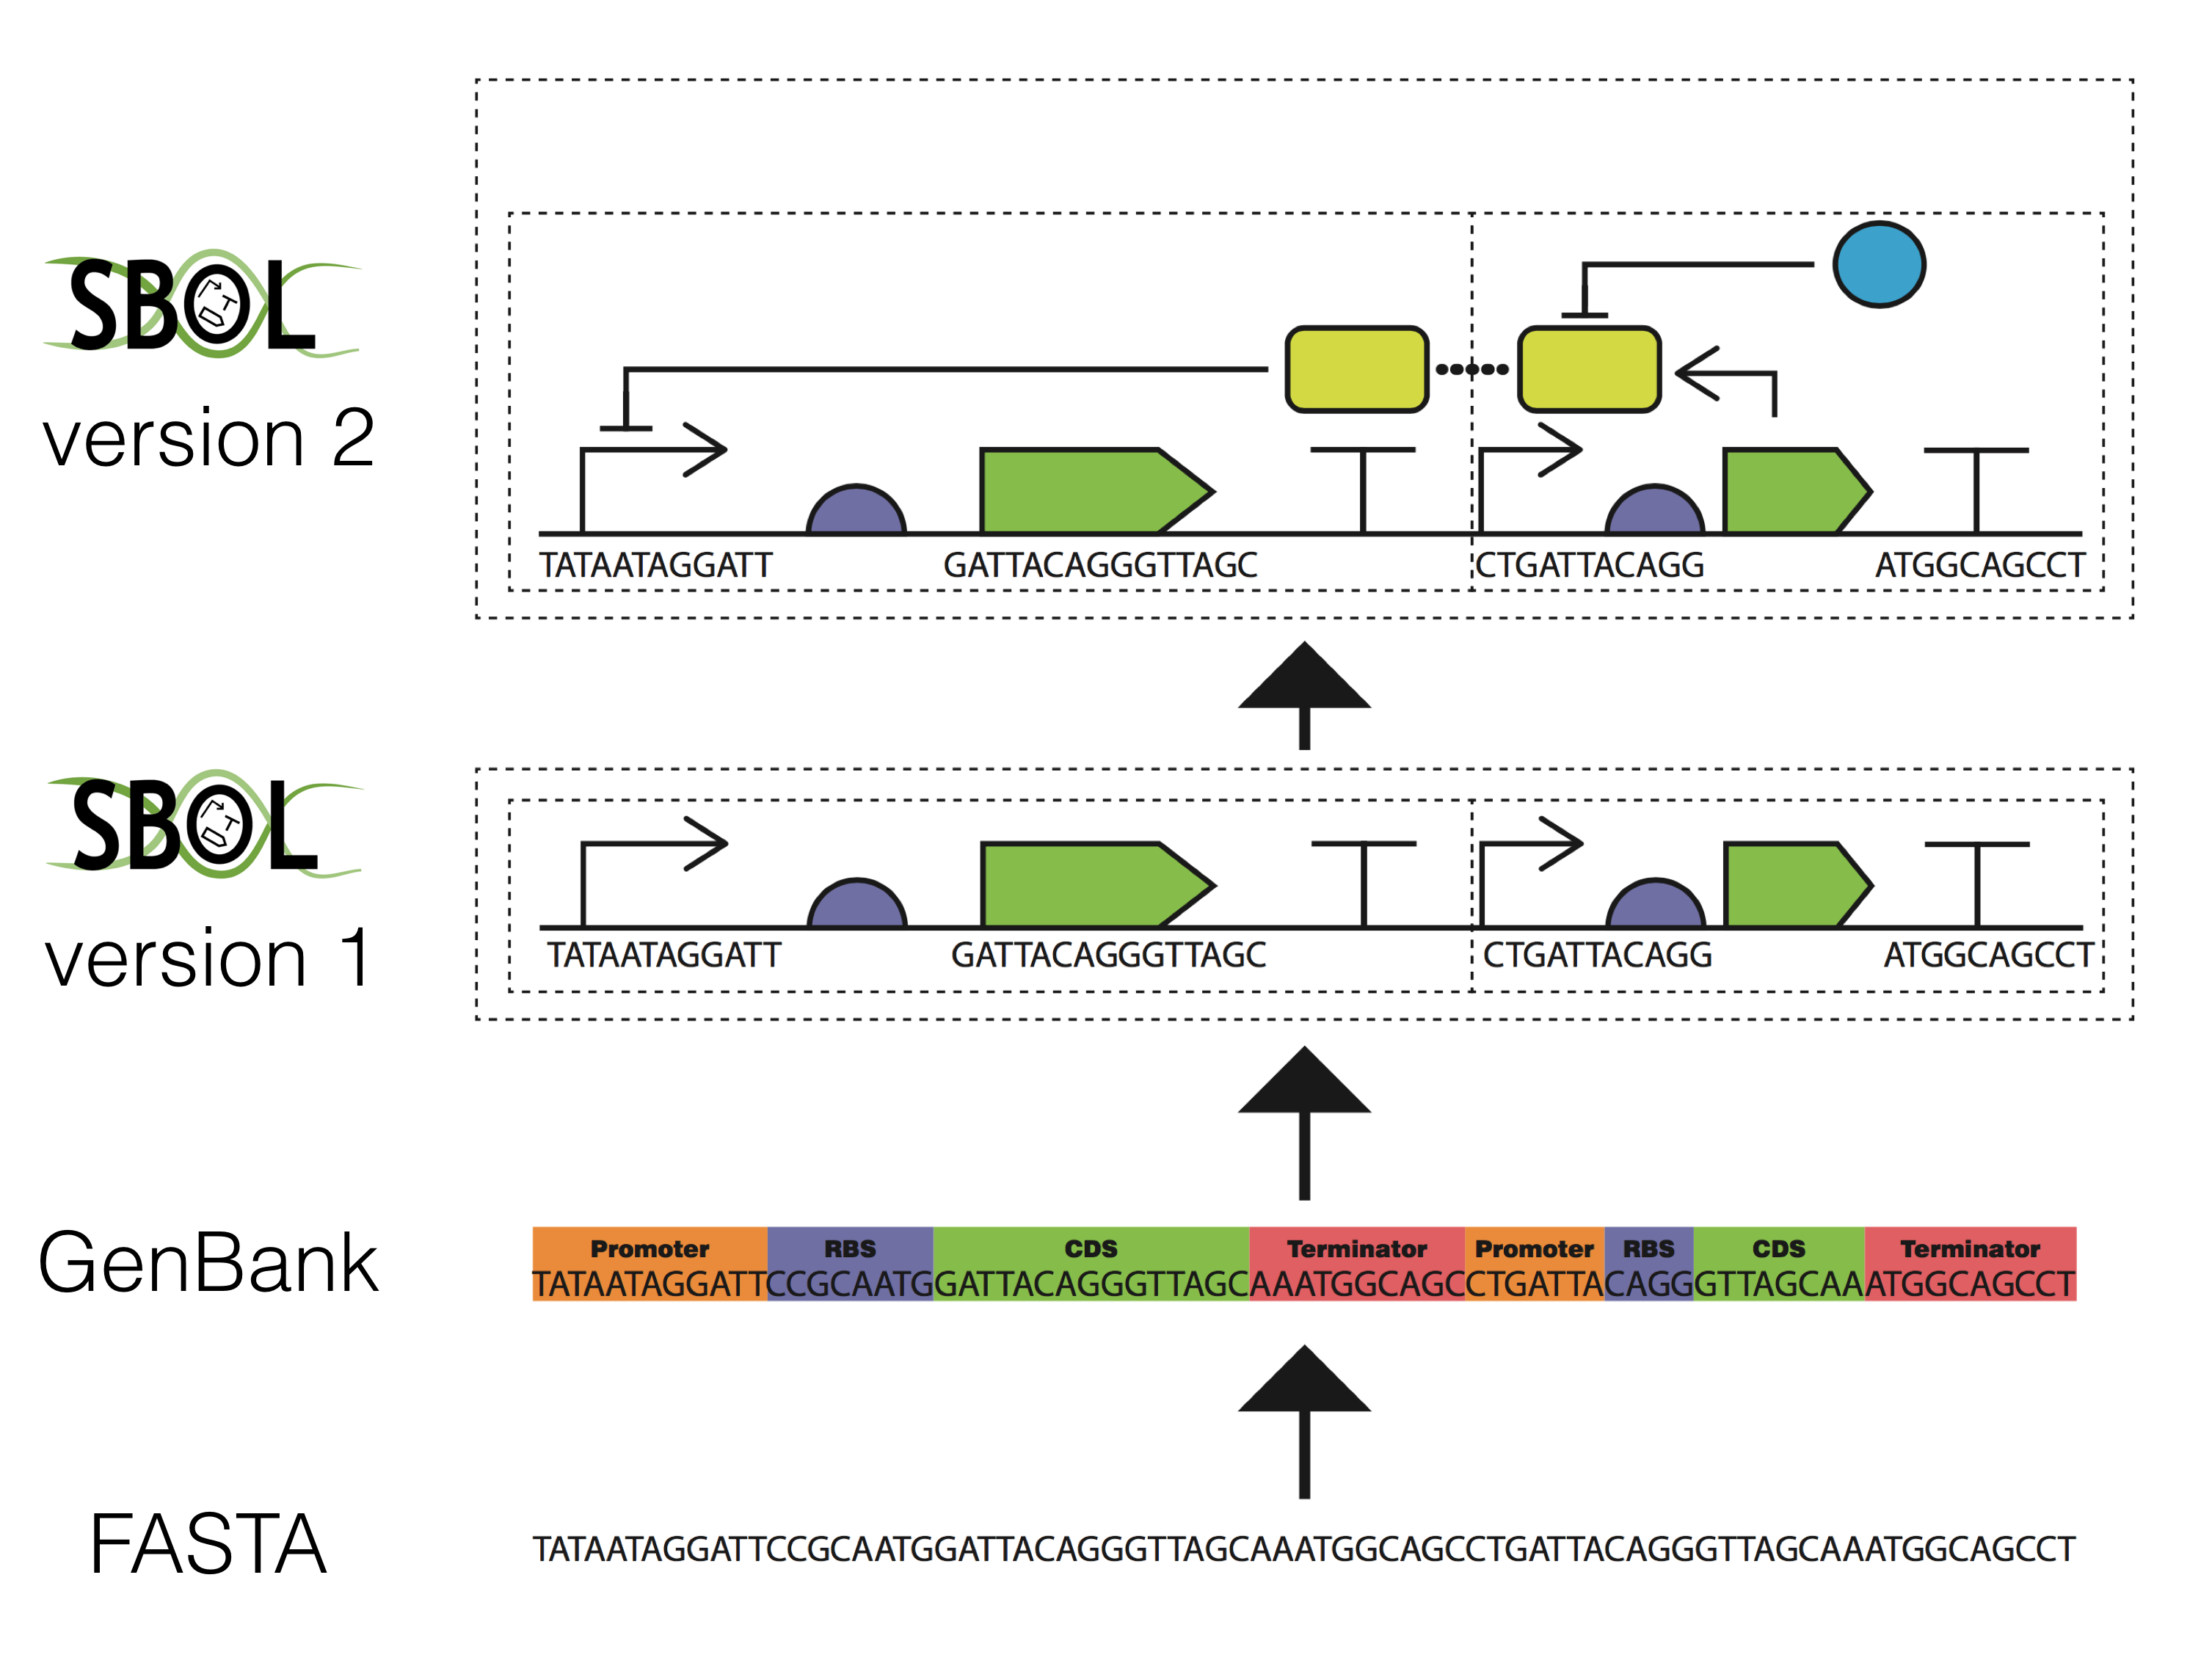
\includegraphics[width=0.75\textwidth]{figs/SBOL}\\
Galdzicki et al., Nature Biotechnology (2014) \\
Roehner et al., ACS Synthetic Biology (2016)
\end{center}
\end{frame}

\begin{frame}\frametitle{Systems Biology Graphical Notation (SBGN)}
\begin{center}
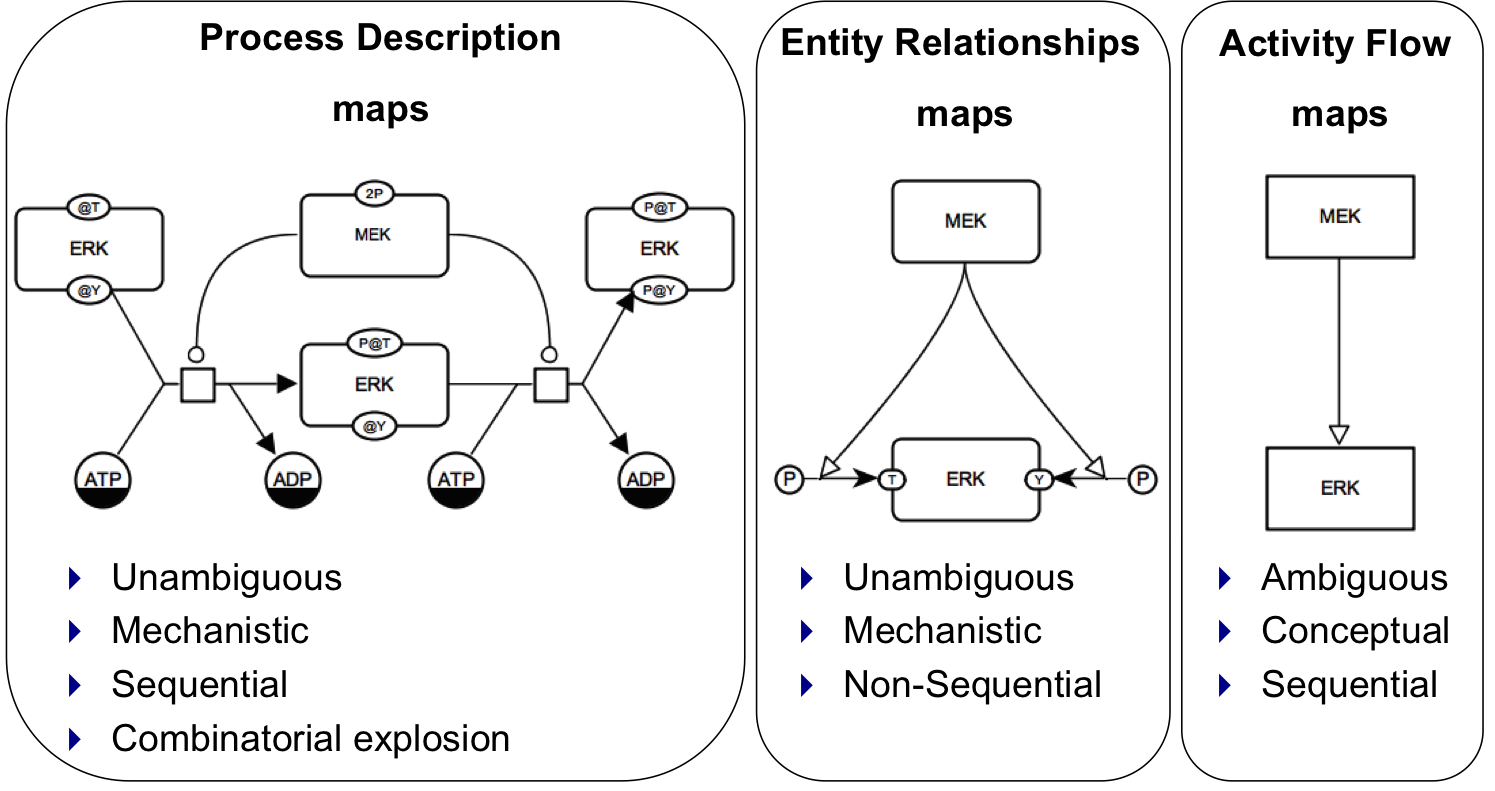
\includegraphics[width=\textwidth]{figs/SBGN2}\\
%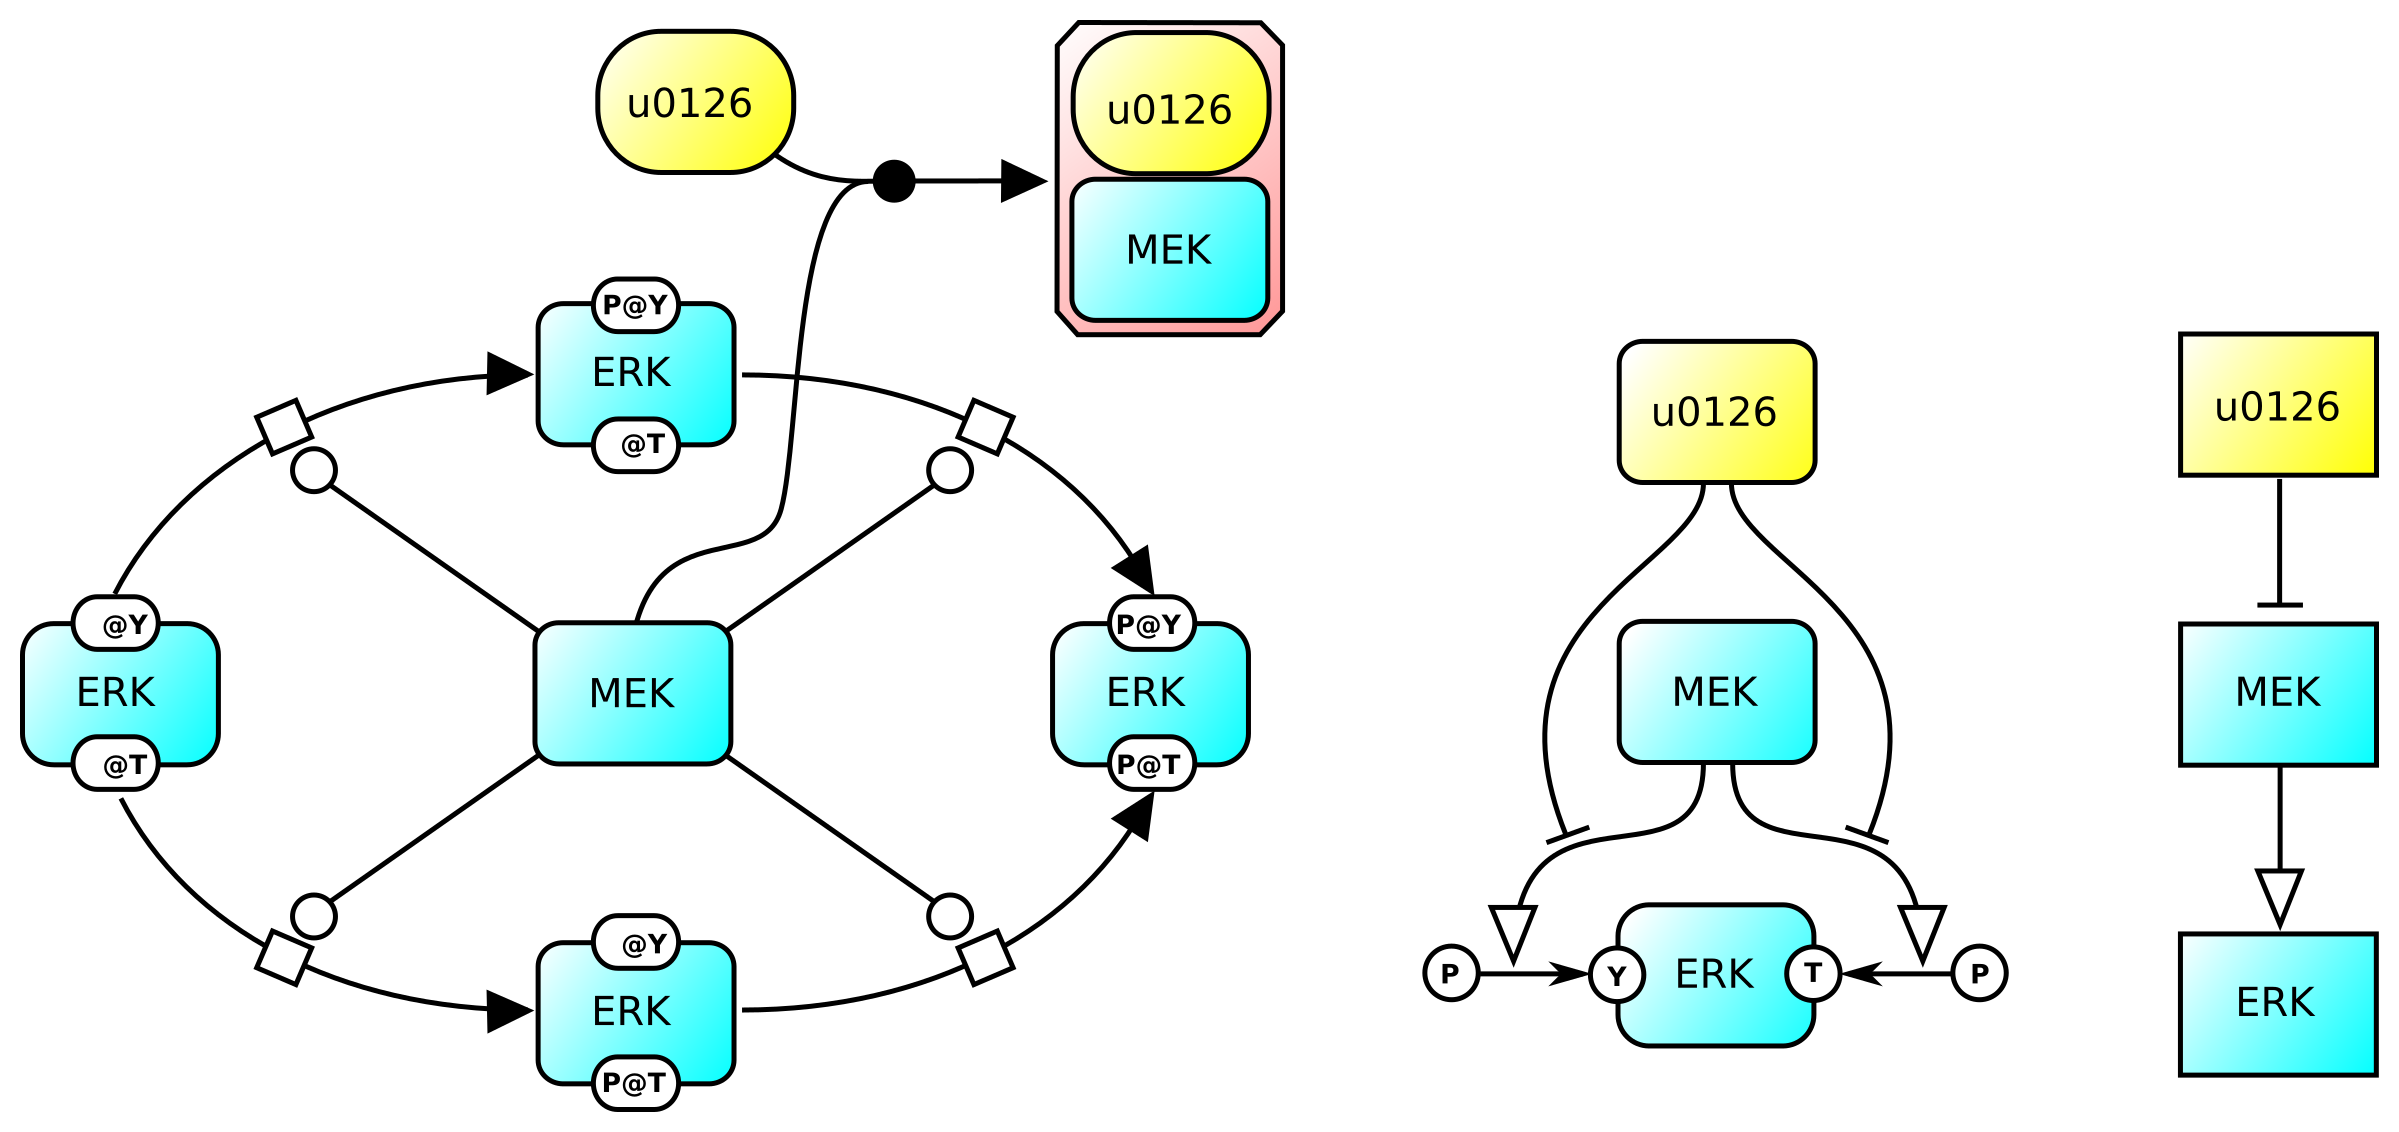
\includegraphics[width=\textwidth]{figs/phosphorylation4-noShadow}\\ 
Le Nov\`{e}re et al., Nature Biotechnology (2009)
\end{center}
\end{frame}

\begin{frame}\frametitle{SBOL Visual (SBOLv)}
\begin{center}
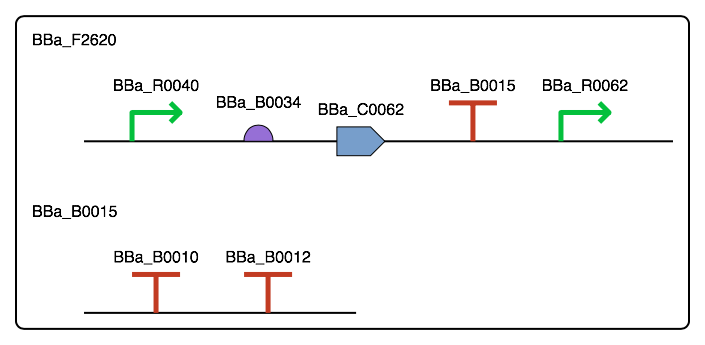
\includegraphics[width=\textwidth]{figs/SBOLExample}\\
Quinn et al., PLoS Biology (2015)
\end{center}
\end{frame}

\begin{frame}\frametitle{Systems Biology Markup Language (SBML)}
\begin{center}
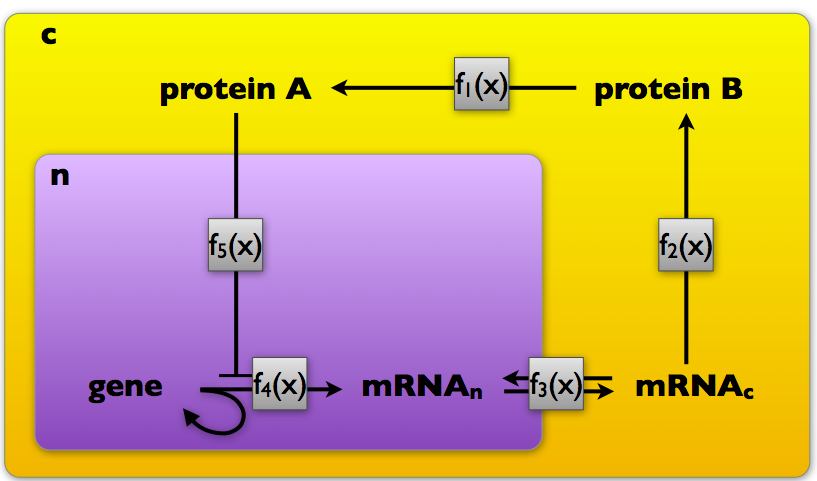
\includegraphics[width=0.45\textwidth]{figs/SBML}\\
Hucka et al., Bioinformatics (2003)
\end{center}
\begin{itemize}
\item Models are composed of a number of species (i.e. proteins, genes, chemical compounds, etc.) and reactions that transform these species.
\item Also include parameters, functions, units, initial assignments, constraints, rules for continuous dynamics, \& events for discontinuous state changes.
%, and constraints to indicate when a simulation should terminate.
\item Biological entities and context are defined mainly via (RDF) annotations.
\item Models can be archived in the BioModels database and/or JWS Online.
\item Supported by more than 280 tools, enabling researchers to create, annotate, simulate, store, exchange, and visualize models.
\end{itemize}
\end{frame}

\begin{frame}\frametitle{CellML}
\begin{center}
\begin{tabular}{cc}
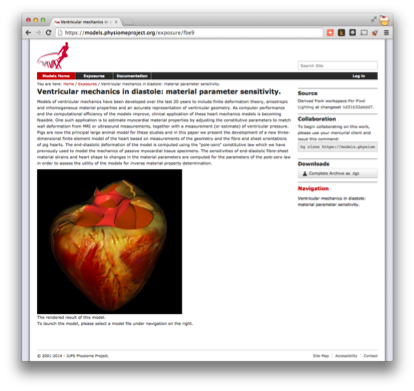
\includegraphics[height=0.3\textheight]{figs/CellML1} &
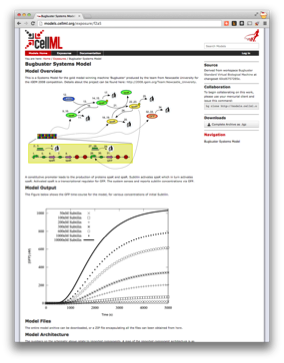
\includegraphics[height=0.3\textheight]{figs/CellML2} 
\end{tabular}\\
Cuellar et al., Simulation (2003)
\end{center}
\begin{itemize}
\item Modular framework for encoding mathematical models:
\begin{itemize}
\item Encodes models consisting of differential algebraic equations w/MathML.
\item Math is the primary data, biological context, provenance, etc., provided through annotations using RDF.
\end{itemize}
\item All quantities require physical units ensuring unambiguous conversion. % of numerical values where required
\item Can define hierarchies of modules to enable mathematical abstraction.
\item External models can be imported enabling reuse.
\item Free and open repository (\url{https://models.physiomeproject.org/}) supporting versioned model reuse, archiving, and collaboration.
\end{itemize}
\end{frame}

\begin{frame}\frametitle{NeuroML: Computational Neuroscience Models}
\begin{center}
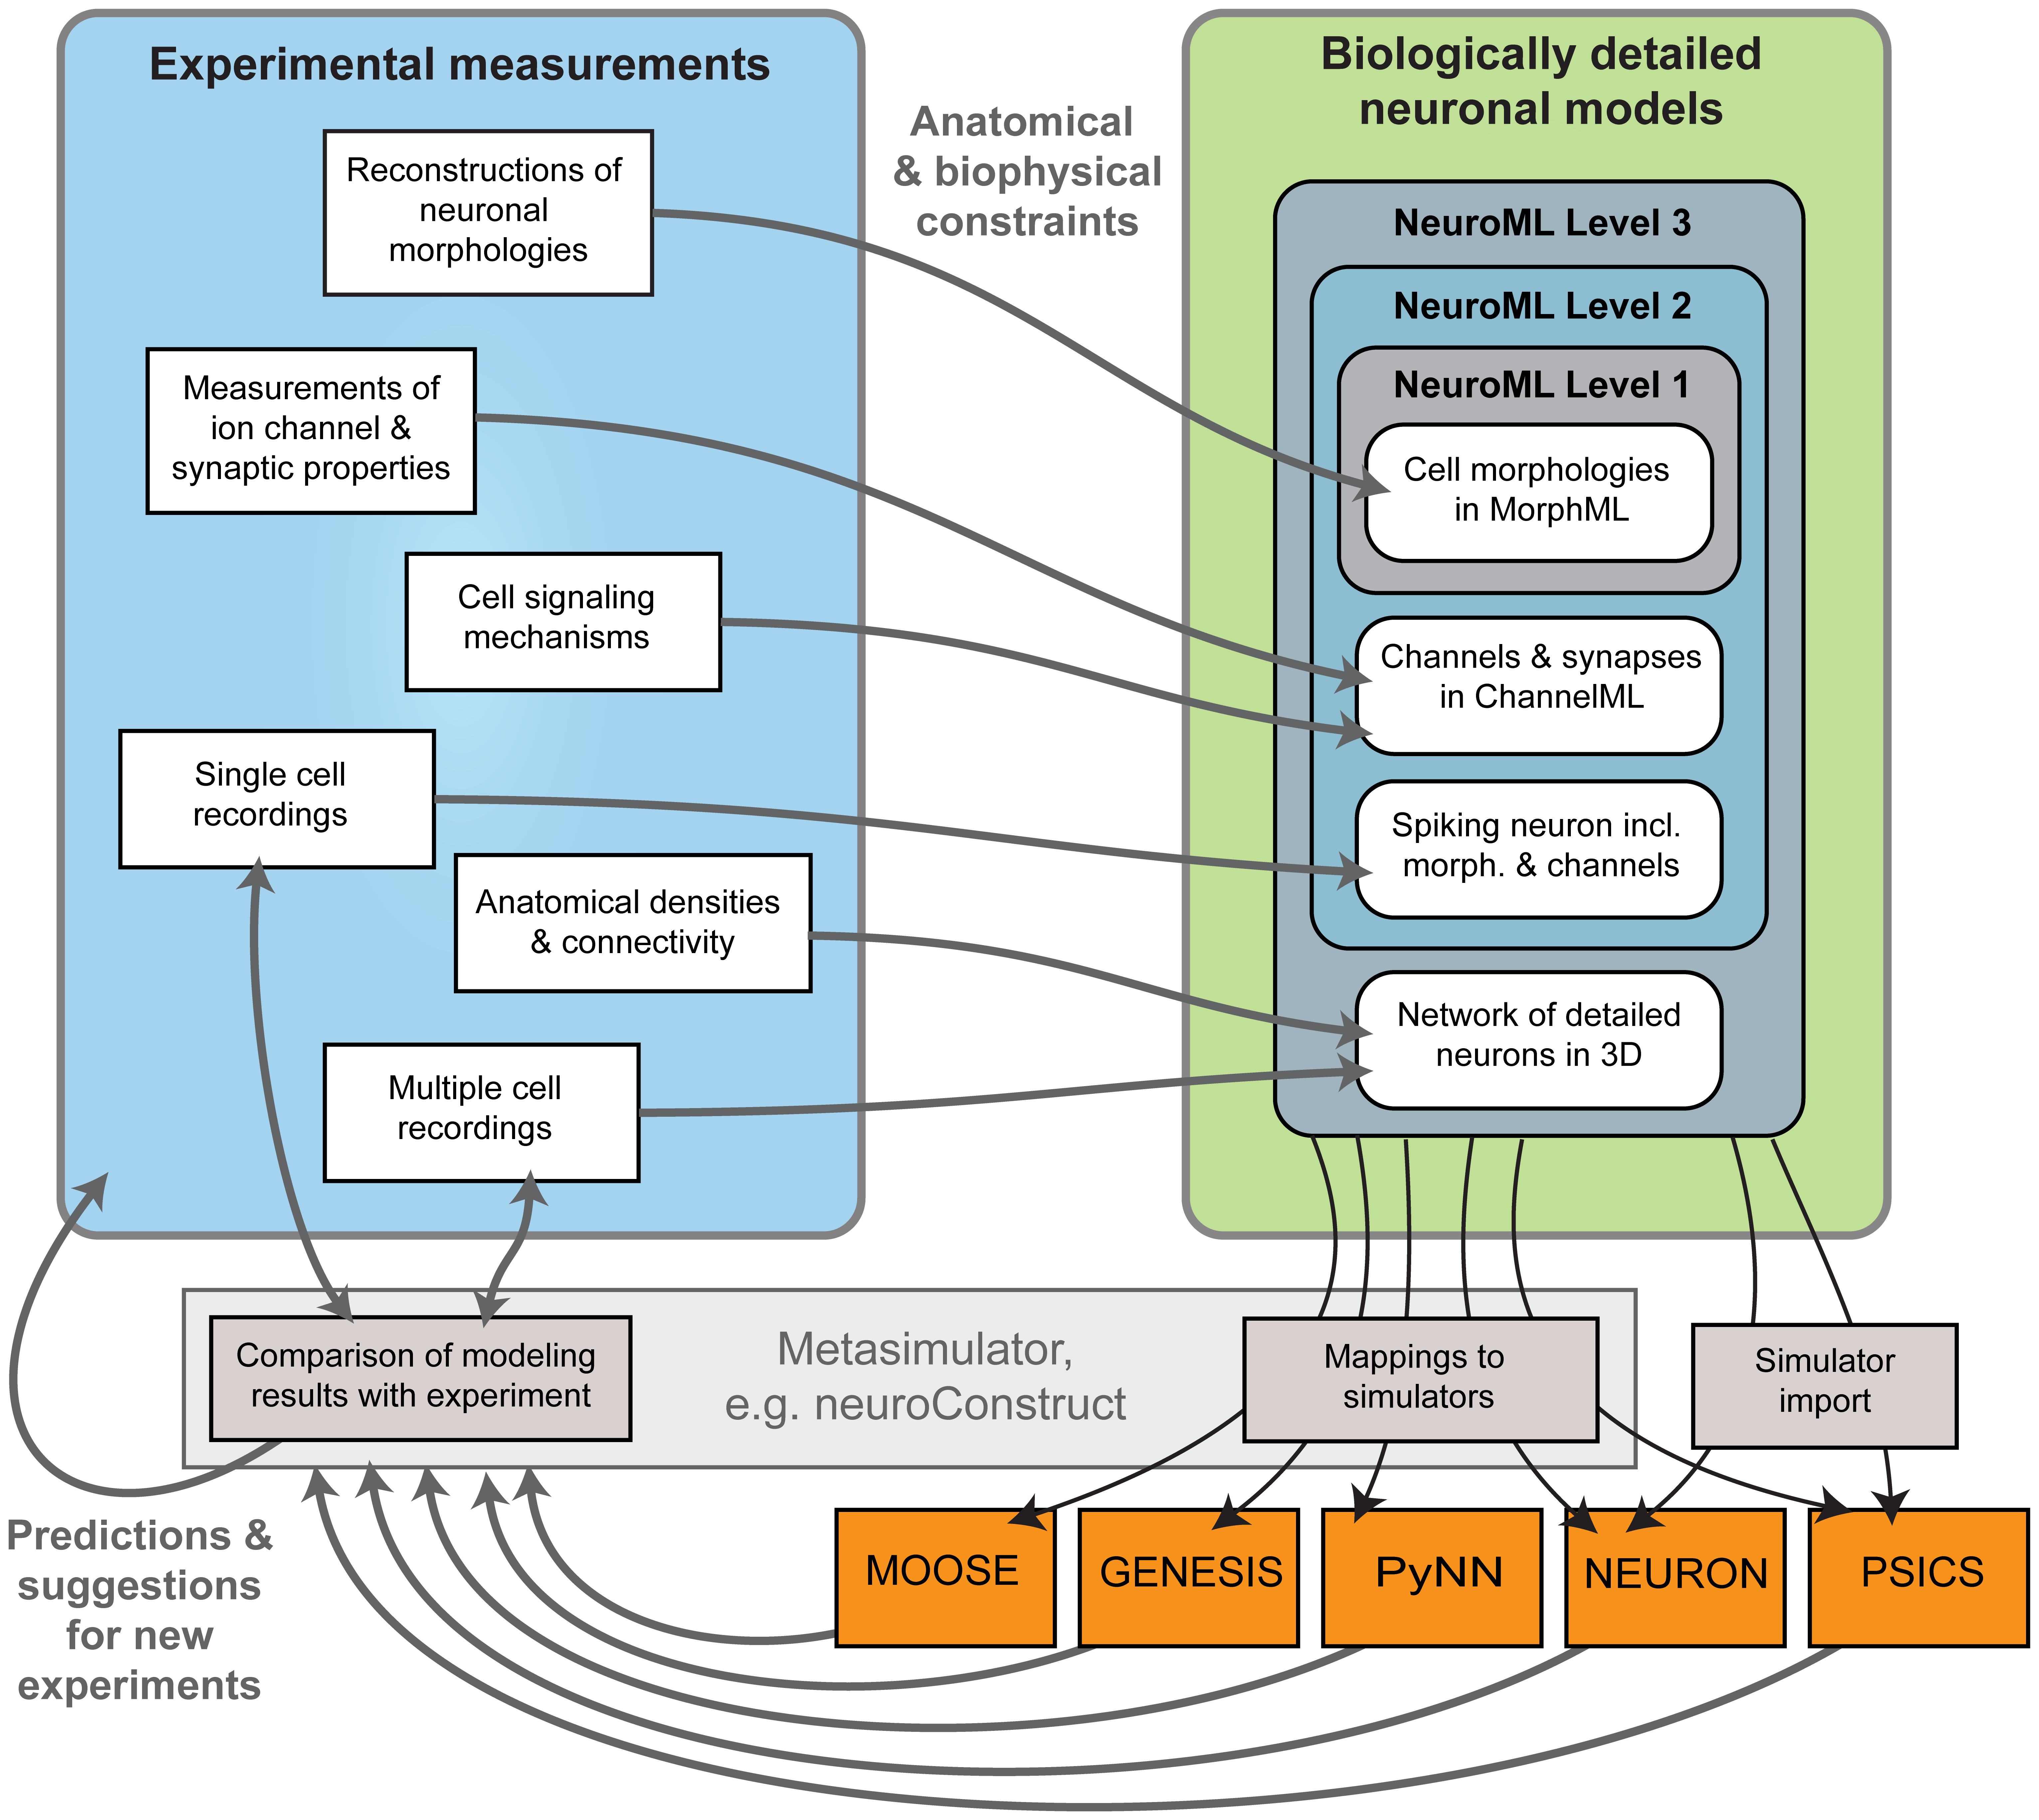
\includegraphics[width=0.65\textwidth]{figs/NeuroML}\\
Gleeson et al., PLoS Computational Biology (2010)
\end{center}
\end{frame}

\begin{frame}\frametitle{Simulation Experiment Description Markup Lang. (SED-ML)}
\begin{center}
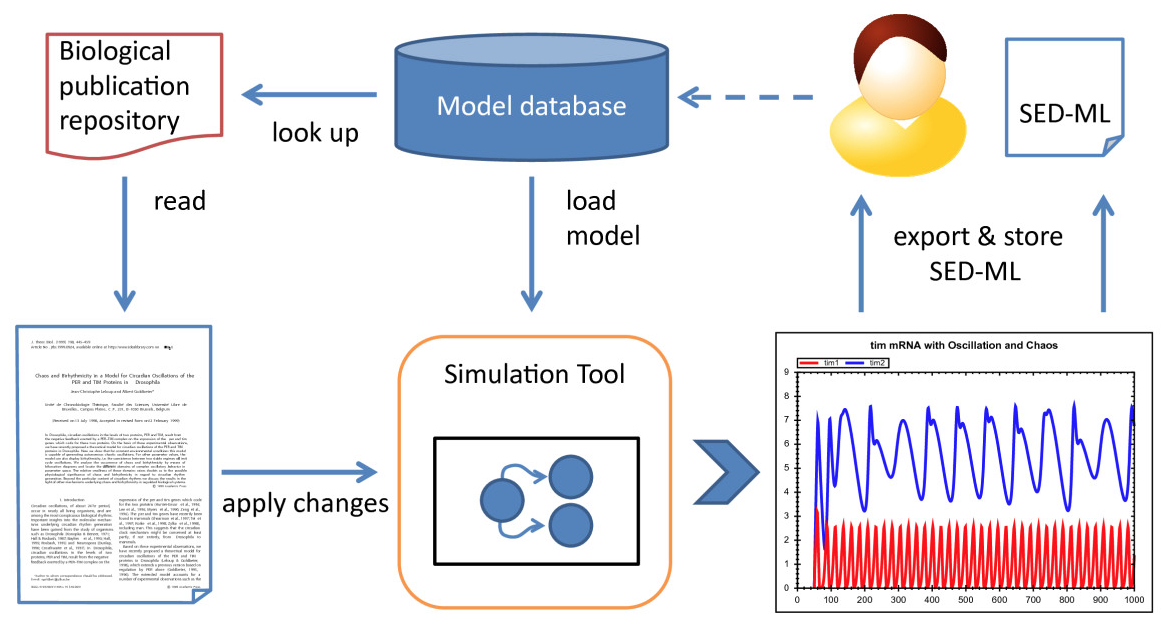
\includegraphics[width=\textwidth]{figs/SED-ML}\\
Waltemath et al., BMC Systems Biology (2011)
\end{center}
\end{frame}

\begin{frame}\frametitle{COMBINE Archive}
\begin{center}
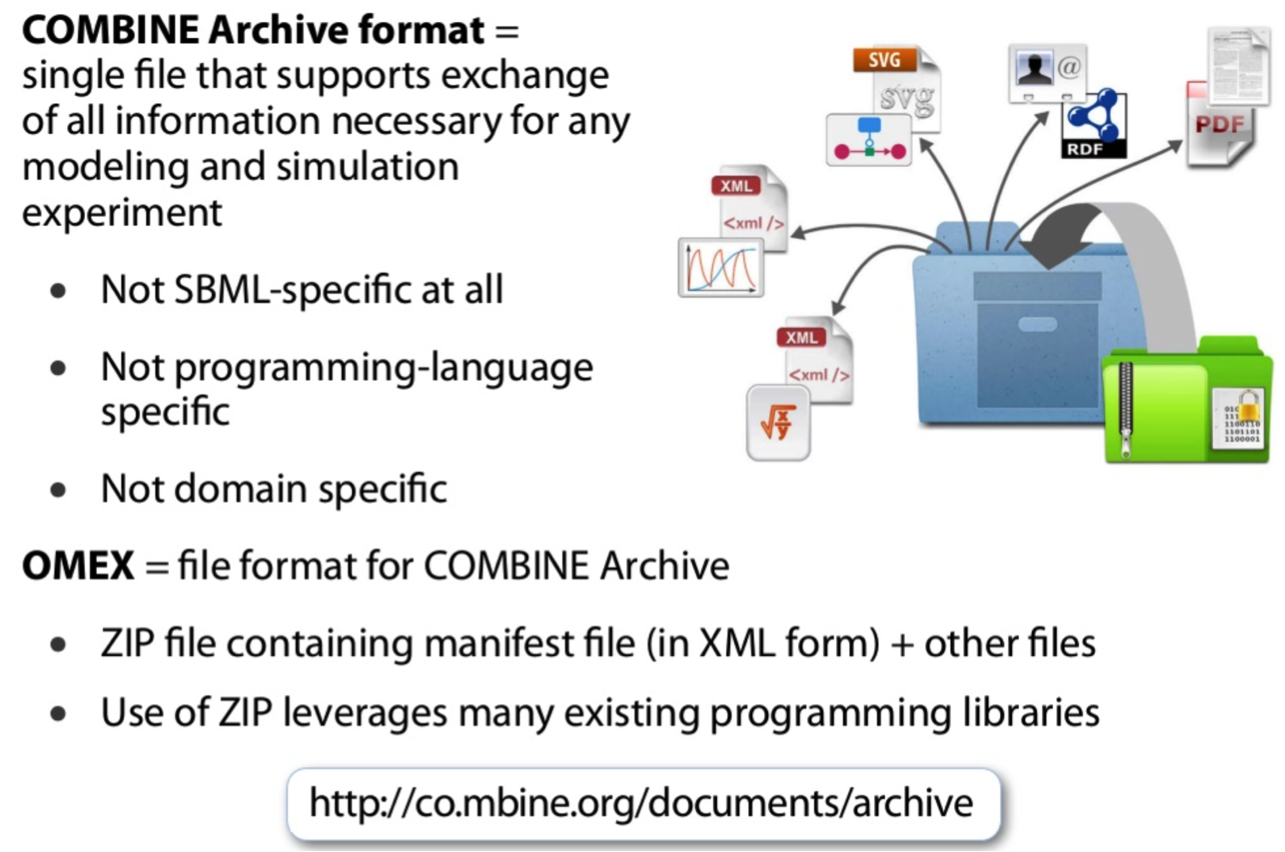
\includegraphics[width=\textwidth]{figs/Archive}
\end{center}
\end{frame}

\begin{frame}\frametitle{Ontologies and Controlled Vocabulary}
\begin{center}
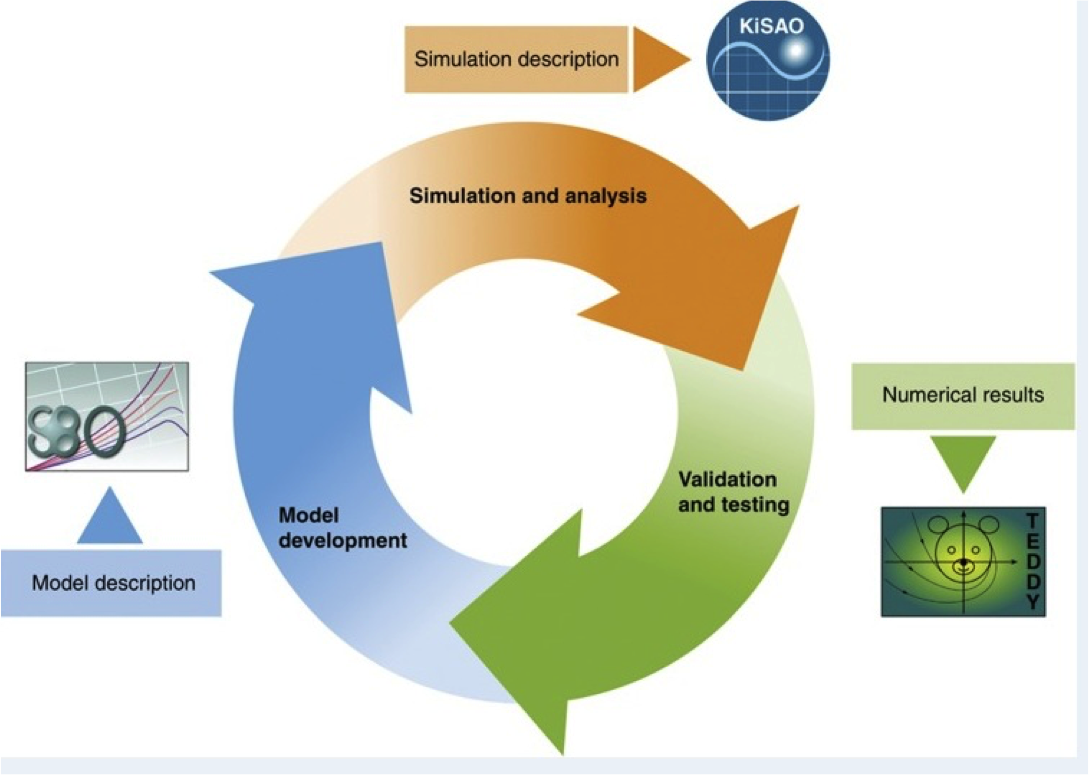
\includegraphics[width=0.85\textwidth]{figs/vocabularies}\\
Courtot, et al., Mol Syst Biol. (2011)
\end{center}
\end{frame}

\begin{frame}\frametitle{Unified Metadata and Annotations}
	\begin{center}
	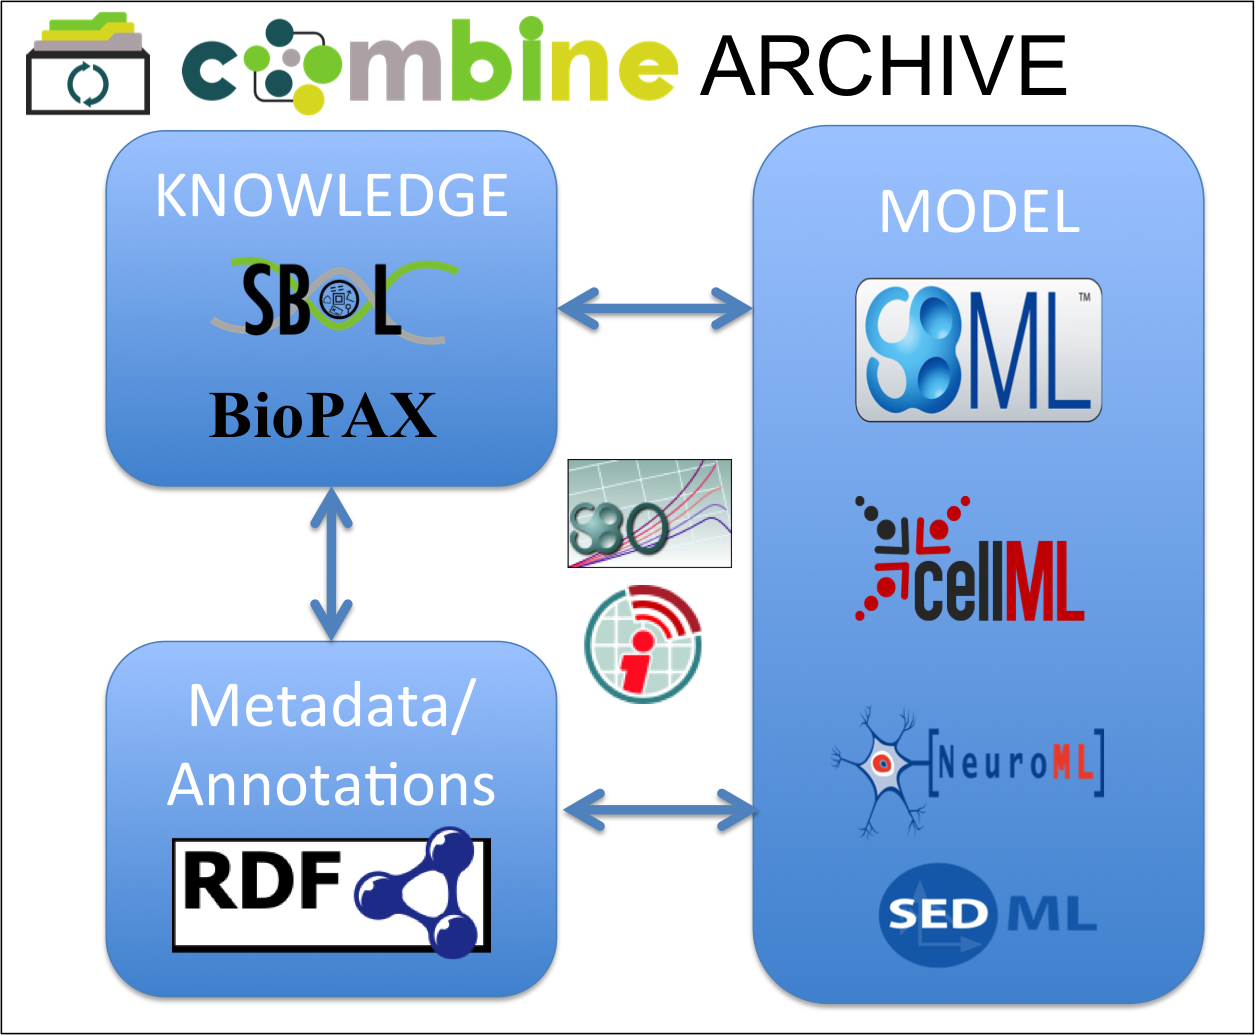
\includegraphics[width=0.75\textwidth]{figs/annotations}
	\end{center}
\end{frame}

\begin{frame}\frametitle{Data Standard Conversions}
	\begin{center}
	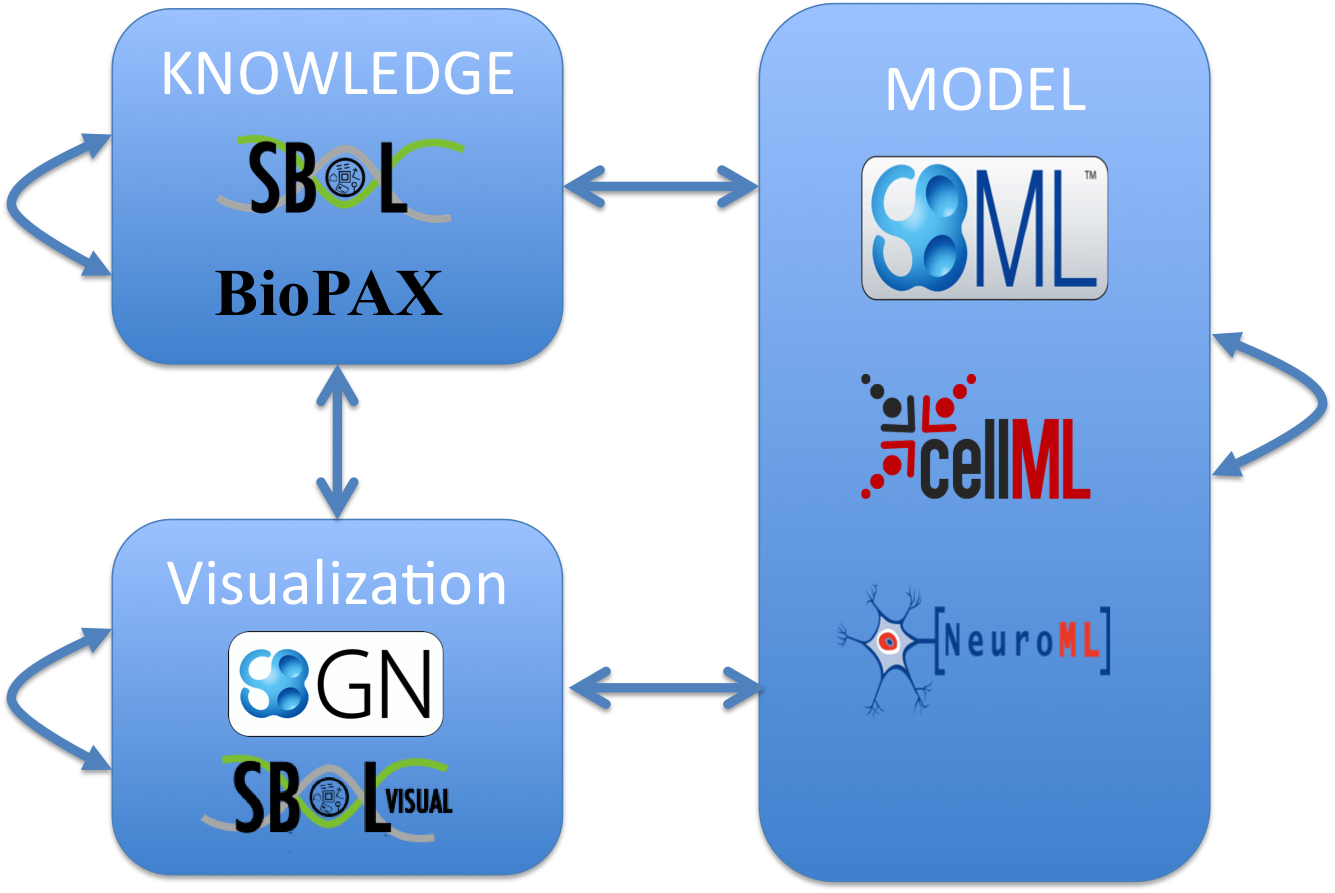
\includegraphics[width=0.9\textwidth]{figs/Conversions}
	\end{center}
\end{frame}

\begin{frame}\frametitle{Interfacing and Interoperability of Standards}
\begin{center}
\includegraphics[width=\textwidth]{figs/interoperability}
\end{center}
\end{frame}

%% \begin{frame}\frametitle{Unified Knowledge Representations (BioPax/SBOL)}
%% \begin{center}
%% % ModuleDefinitions -> Pathways
%% % Interactions -> Interactions (SBO)
%% % ComponentDefinitions (BioPax Types) -> PhysicalEntities
%% \end{center}
%% \end{frame}

\begin{frame}\frametitle{Unified Visualizations (SBGN/SBOLv)}
\begin{center}
\only<1>{
\begin{tabular}{cc}
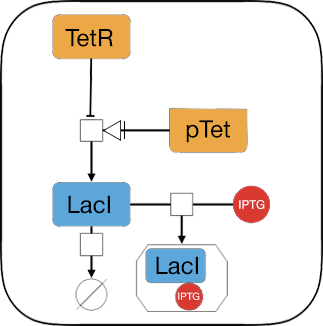
\includegraphics[width=0.45\textwidth]{figs/SBML_iilus.png} &
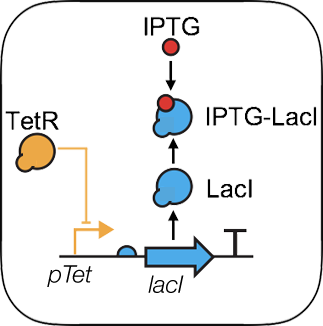
\includegraphics[width=0.45\textwidth]{figs/SBOL_illus.png} \\
SBGN & SBOLv
\end{tabular}
}
\only<2>{
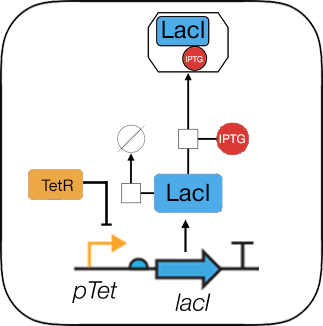
\includegraphics[width=0.55\textwidth]{figs/hybrid_illus.png}\\
Unified SBGN/SBOLv
}
\end{center}
\end{frame}

\begin{frame}\frametitle{Repositories}
\begin{center}
{\scriptsize
\begin{tabular}{cc}
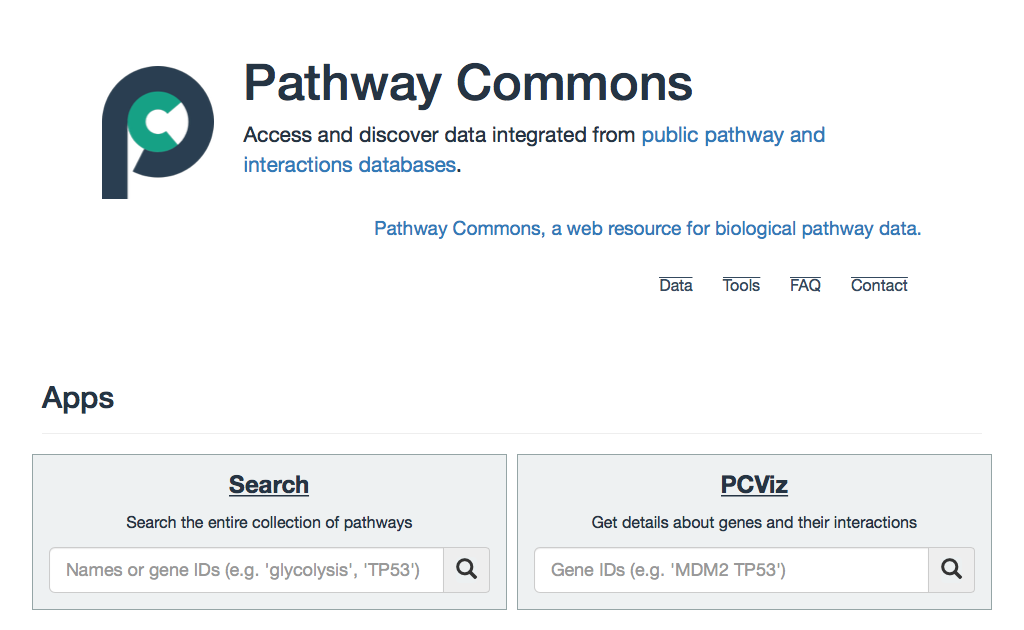
\includegraphics[width=0.375\textwidth]{figs/pathwayCommons} & 
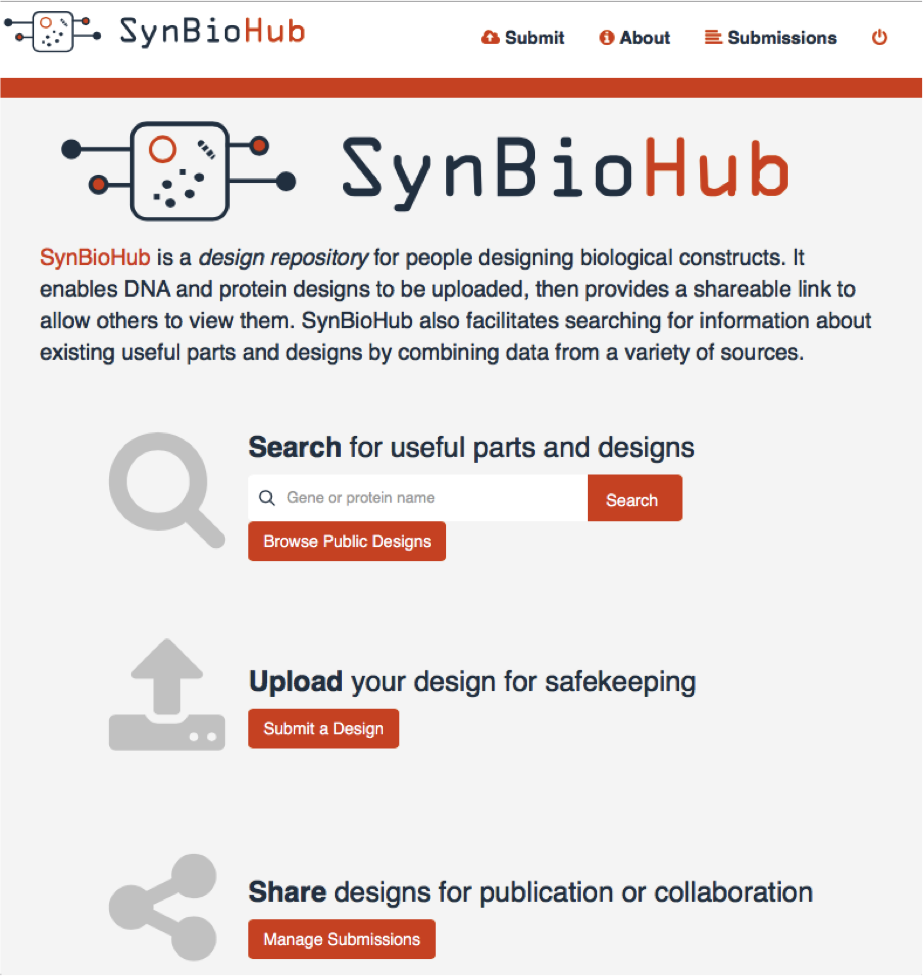
\includegraphics[width=0.3\textwidth]{figs/synBioHub1} \\
\url{http://www.pathwaycommons.org} & \url{https://synbiohub.org} \\
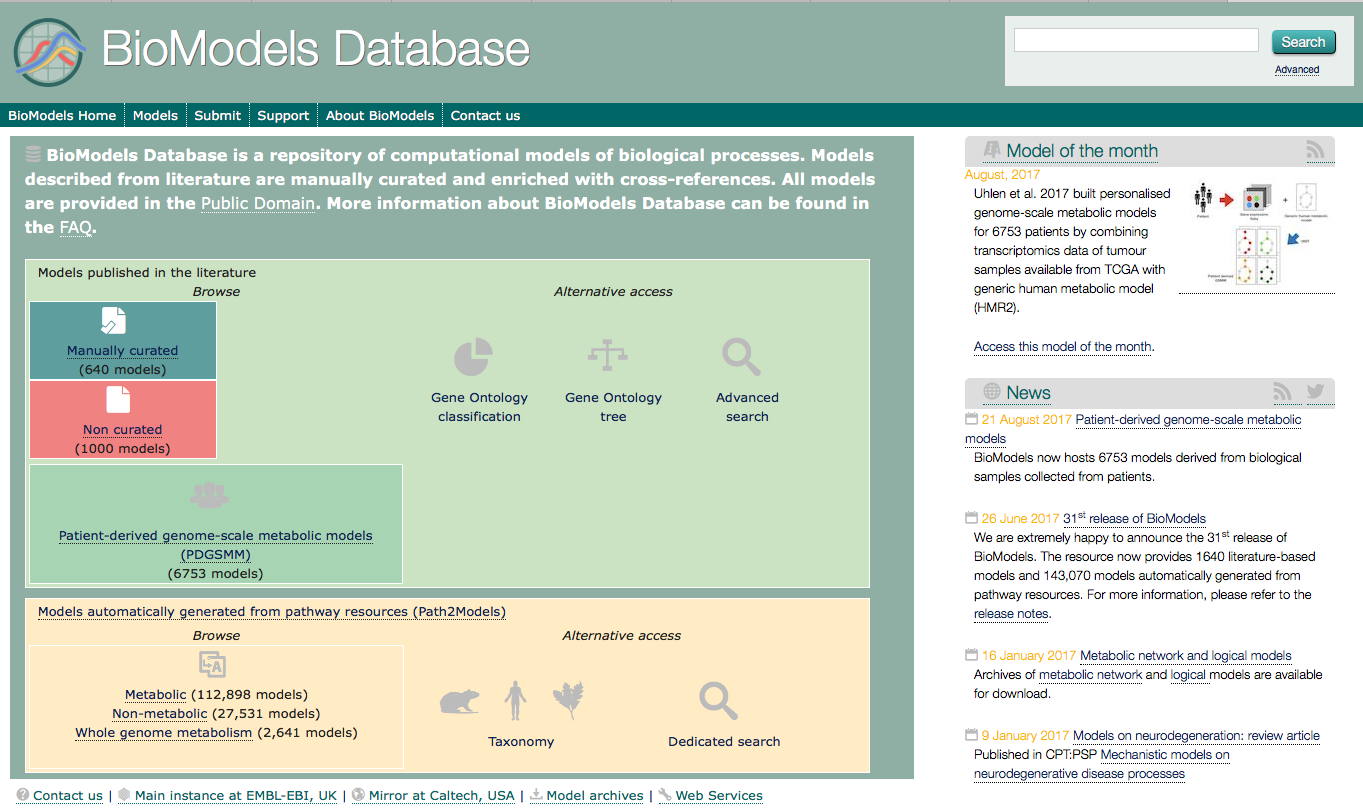
\includegraphics[width=0.375\textwidth]{figs/BioModels} &
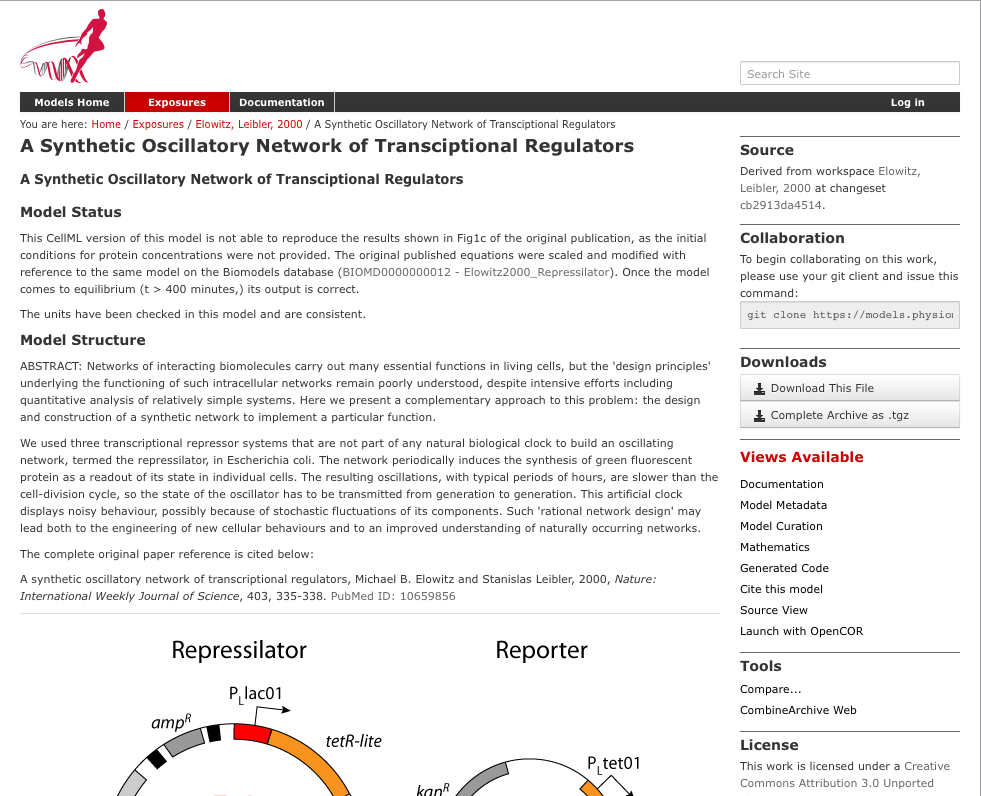
\includegraphics[width=0.3\textwidth]{figs/physiome} \\
\url{http://biomodels.net} & \url{https://models.physiomeproject.org}
\end{tabular}
}
\end{center}
\end{frame}

%% \begin{frame}\frametitle{Ongoing Projects and Future Opportunities}
%% \begin{center}
%% %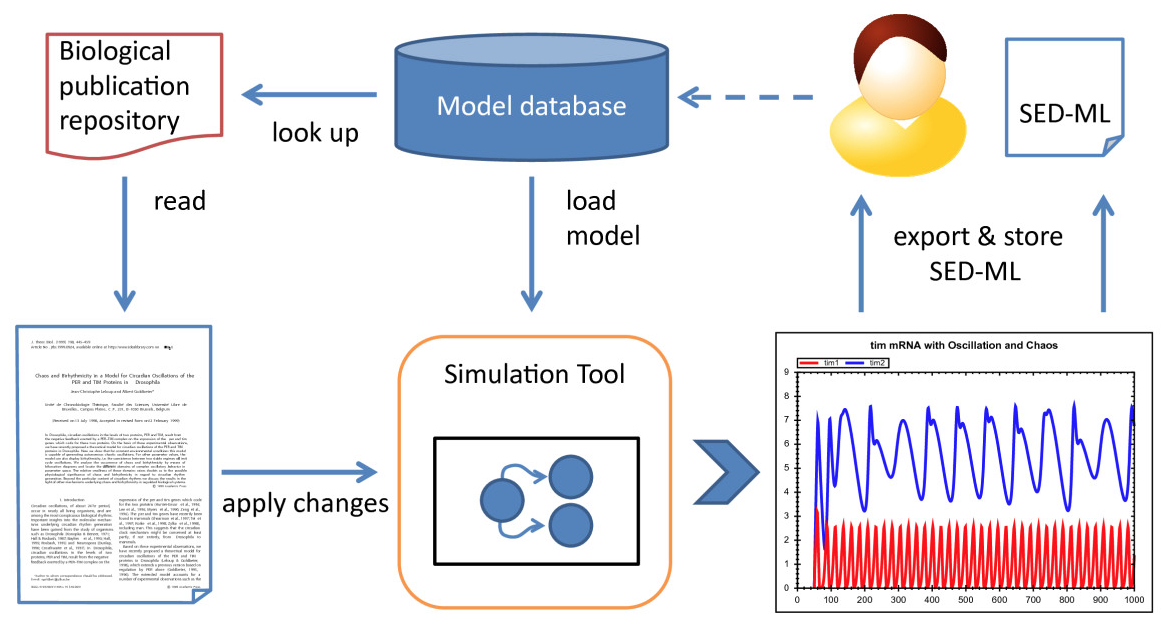
\includegraphics[width=\textwidth]{figs/SED-ML}
%% \end{center}
%% \end{frame}

%% \begin{frame}\frametitle{Unified Modeling Standards (SBML/CellML/SBOL/SED-ML)}
%% \begin{center}
%% \end{center}
%% \end{frame}

\begin{frame}\frametitle{Standard Enabled System/Synthetic Biology Workflows}
\begin{center}
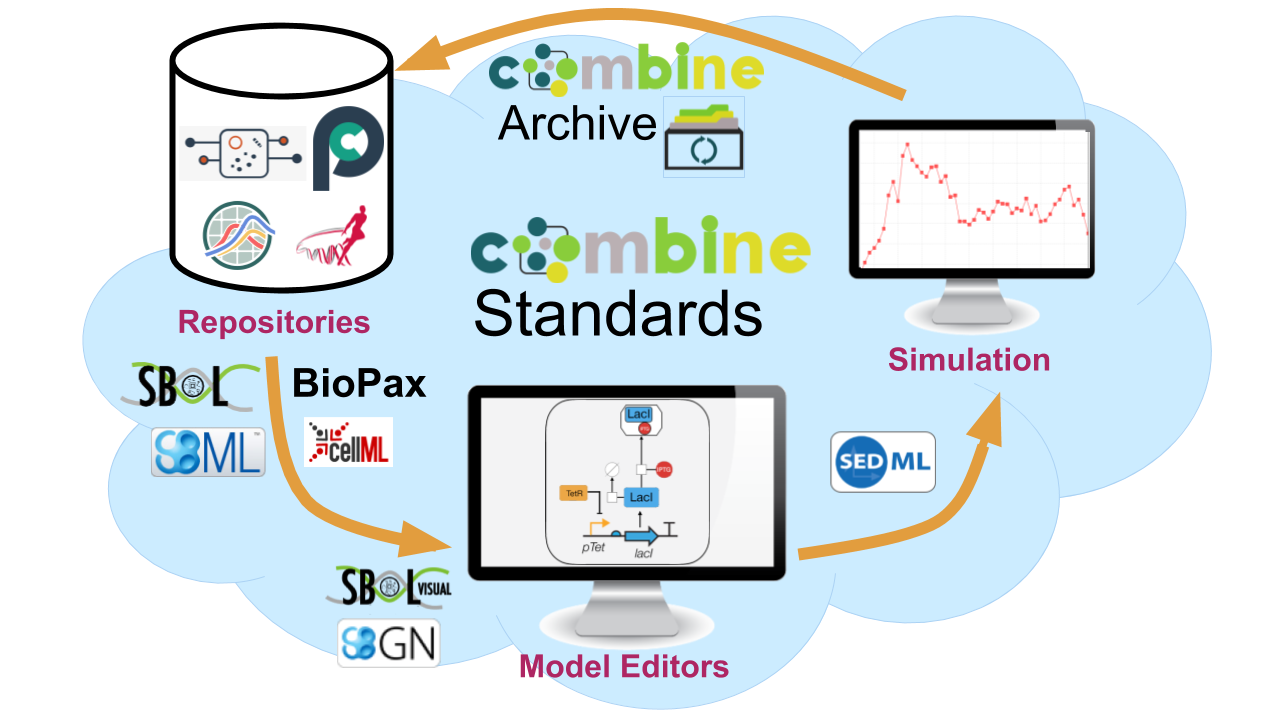
\includegraphics[width=\textwidth]{figs/COMBINE_workflow2}
\end{center}
\end{frame}

\begin{frame}\frametitle{Journal Workflow for Reproducibility}
\begin{center}
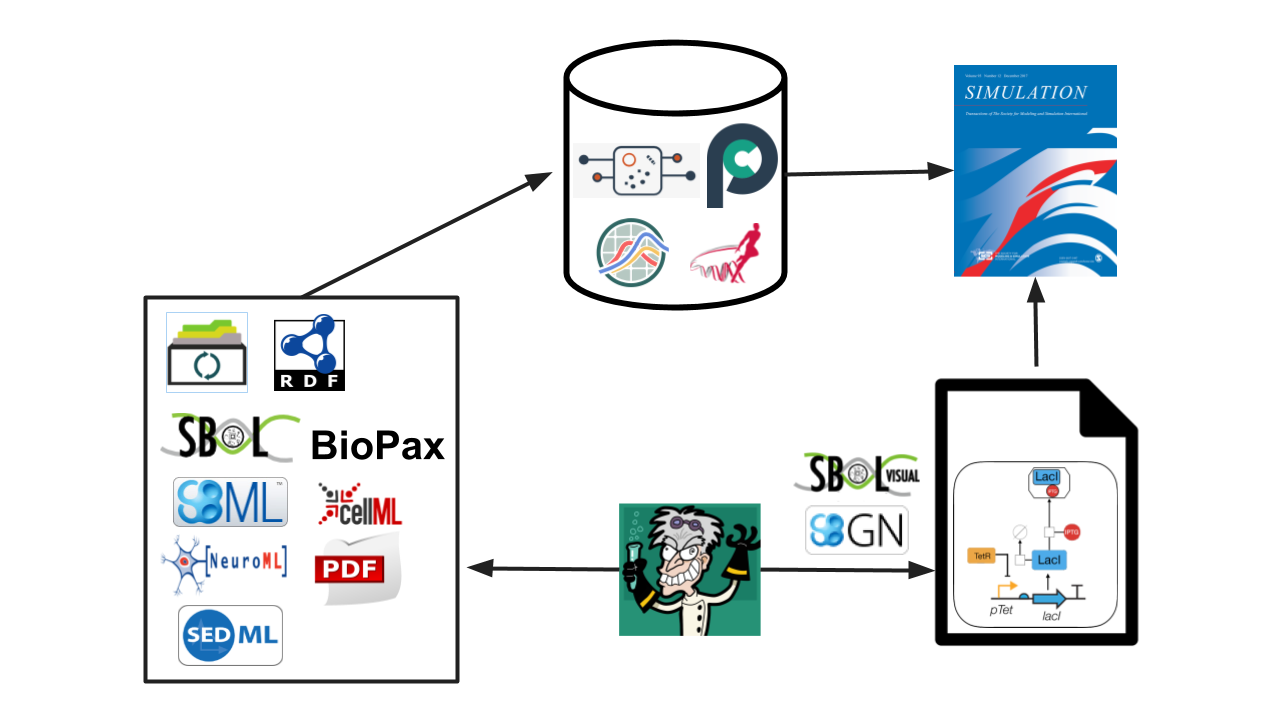
\includegraphics[width=\textwidth]{figs/JournalFlow}
\end{center}
\end{frame}

\begin{frame}\frametitle{Conclusion}
\begin{quotation}
While reproducibility remains a challenge in computational modeling in biology, the COMBINE community and the standards being developed within this community have the potential to make this a fully reproducible scientific endeavor.
\end{quotation}
\end{frame}

\begin{frame}\frametitle{COMBINE Coordination Board}
\begin{center}
\only<1>{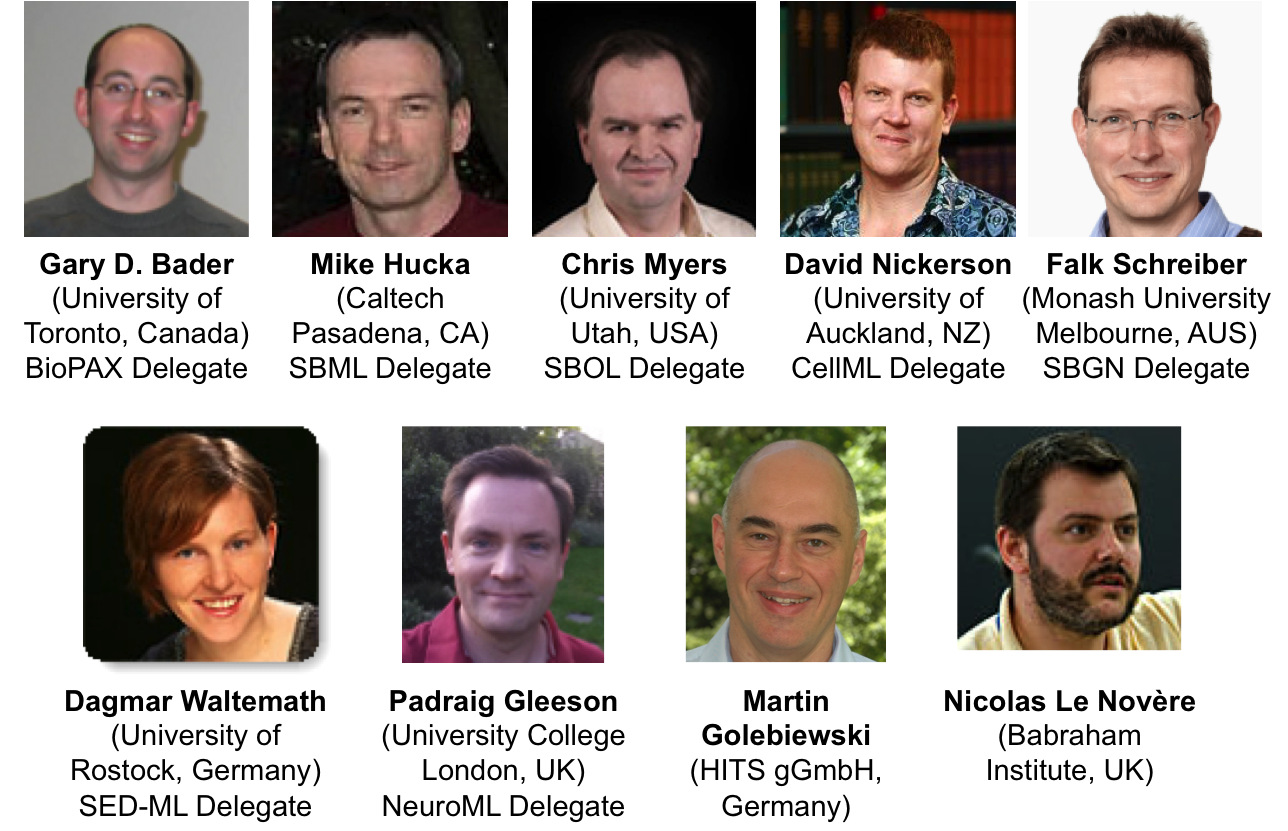
\includegraphics[width=\textwidth]{figs/BoardOld}}
\only<2>{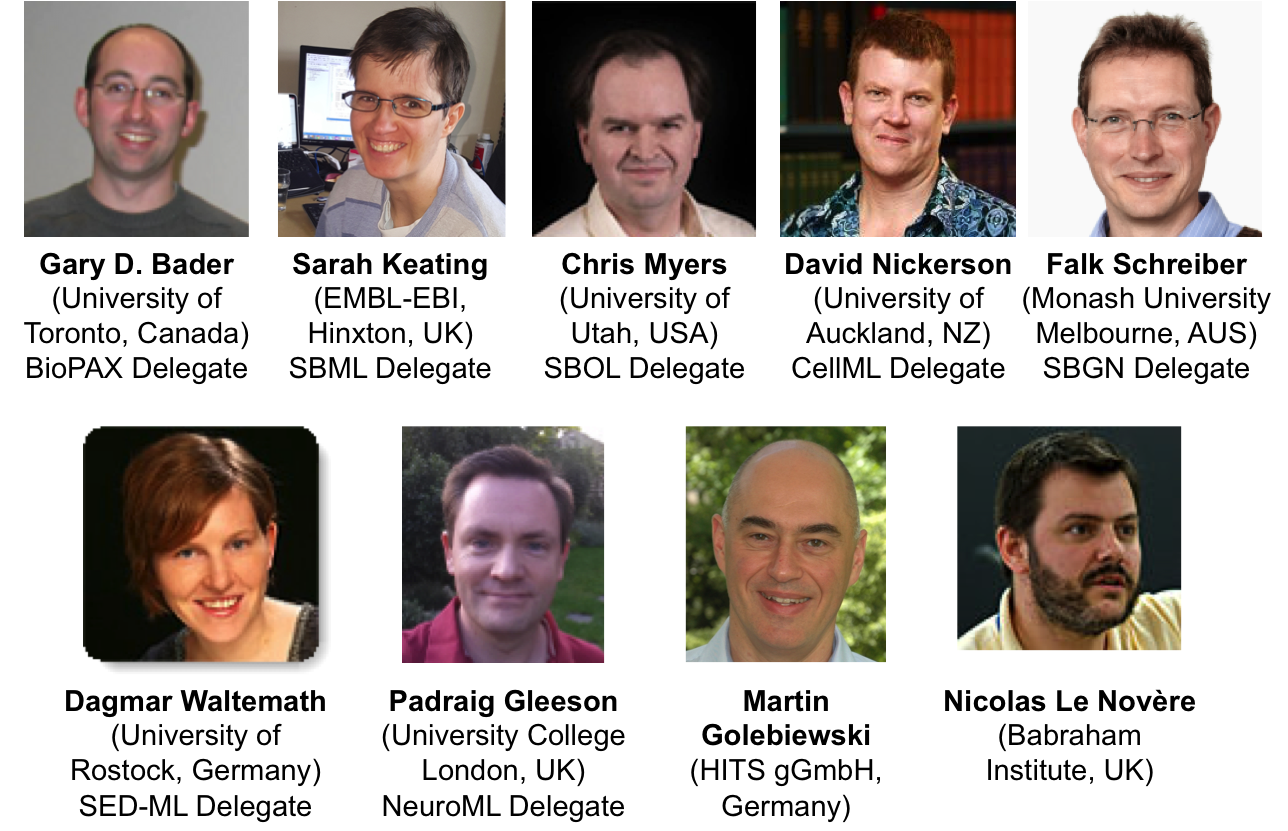
\includegraphics[width=\textwidth]{figs/Board}}
\end{center}
\end{frame}

\begin{frame}\frametitle{Invitation}
\begin{itemize}
\item You are invited to join the COMBINE community.
\item Contact the COMBINE Coordinators or standard editors to join the appropriate mailing lists.
\item Attend our upcoming events:
\end{itemize}
\begin{center}
\begin{tabular}{cc}
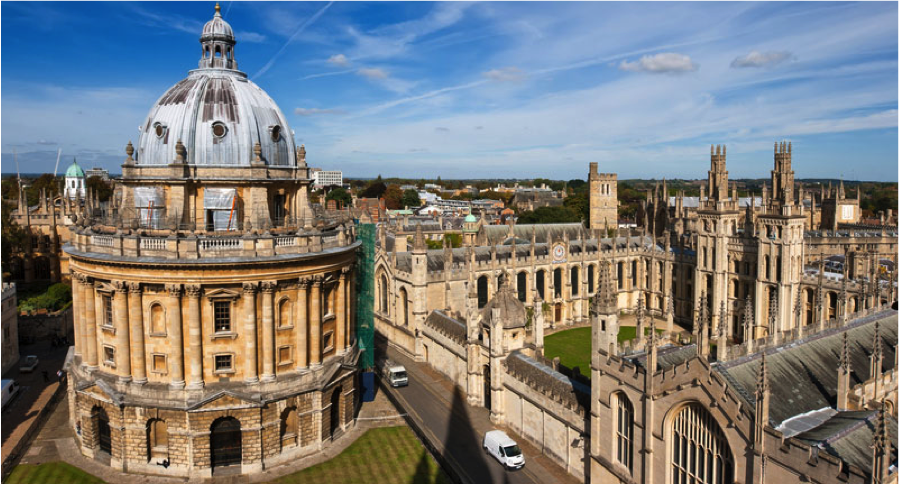
\includegraphics[width=0.55\textwidth]{figs/Oxford} &
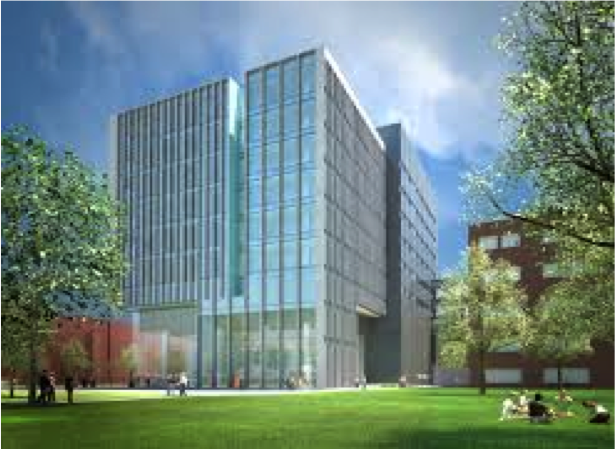
\includegraphics[width=0.4\textwidth]{figs/BU} \\
HARMONY 2018 & COMBINE Forum 2018 \\
University of Oxford & Boston University \\
 June 18-22 & October 8-12
\end{tabular}
\end{center}
\end{frame}

\end{document}


